\documentclass[11pt,a4paper]{article}
\usepackage[utf8]{inputenc}
\usepackage[T1]{fontenc}
\usepackage{mathpazo}
\usepackage{graphicx, graphics, epsfig, color}
\usepackage{booktabs}
\usepackage{subcaption}
\usepackage{amsmath,amssymb,amsthm}
\usepackage{tikz, pgfplots}
\usetikzlibrary{plotmarks}
\pgfplotsset{compat=newest}
\usepackage[margin=3cm]{geometry}
\usepackage{hyperref}
\hypersetup{colorlinks=false}
\usepackage{cleveref}

% math operator
\DeclareMathOperator{\tr}{tr}
\DeclareMathOperator{\diag}{diag}
\DeclareMathOperator{\rank}{rank}
\DeclareMathOperator{\Cov}{Cov}
\DeclareMathOperator{\Res}{Res}
\DeclareMathOperator{\supp}{supp}
\DeclareMathOperator{\dist}{dist}
\newcommand{\T}{{\sf T}}
\renewcommand{\H}{{\sf H}}
\DeclareMathOperator*{\argmin}{arg\,min}

\newcommand{\RR}{{\mathbb{R}}}
\newcommand{\CC}{{\mathbb{C}}}
\newcommand{\EE}{{\mathbb{E}}}
\newcommand{\NN}{{\mathcal{N}}}
%
%
%
\newcommand{\A}{{\mathbf{A}}}
\newcommand{\B}{{\mathbf{B}}}
\newcommand{\C}{{\mathbf{C}}}
\newcommand{\J}{{\mathbf{J}}}
\newcommand{\M}{{\mathbf{M}}}
\renewcommand{\S}{{\mathbf{S}}}
\renewcommand{\P}{{\mathbf{P}}}
\newcommand{\U}{{\mathbf{U}}}
\newcommand{\Q}{{\mathbf{Q}}}
\newcommand{\X}{{\mathbf{X}}}
\newcommand{\Z}{{\mathbf{Z}}}
\newcommand{\bPhi}{{\boldsymbol{\Phi}}}
%
%
%
\newcommand{\ee}{\mathbf{e}}
\newcommand{\uu}{\mathbf{u}}
\newcommand{\vv}{\mathbf{v}}

\newcommand{\s}{\mathbf{s}}
\newcommand{\x}{\mathbf{x}}
\newcommand{\y}{\mathbf{y}}
\newcommand{\z}{\mathbf{z}}
\newcommand{\zo}{\mathbf{0}}
\newcommand{\I}{\mathbf{I}}
\newcommand{\V}{\mathbf{V}}


\newcommand{\bLambda}{\boldsymbol{\Lambda}}
\newcommand{\bomega}{\boldsymbol{\omega}}
\newcommand{\bepsilon}{{\boldsymbol{\epsilon}}}

\newcommand{\cd}{{ \xrightarrow{d} }}
\newcommand{\asto}{{ \xrightarrow{a.s.} }}

% define color
\definecolor{RED}{rgb}{0.7,0,0}
\definecolor{BLUE}{rgb}{0,0,0.69}
\definecolor{GREEN}{rgb}{0,0.6,0}
\definecolor{PURPLE}{rgb}{0.69,0,0.8}

%text color
\newcommand{\RED}{\color[rgb]{0.70,0,0}}
\newcommand{\BLUE}{\color[rgb]{0,0,0.69}}
\newcommand{\GREEN}{\color[rgb]{0,0.6,0}}
\newcommand{\PURPLE}{\color[rgb]{0.69,0,0.8}}

% theorems
\newtheorem{Definition}{Definition}
\newtheorem{Assumption}{Assumption}
\newtheorem{Theorem}{Theorem}
\newtheorem{Corollary}{Corollary}
\newtheorem{Proposition}{Proposition}
\newtheorem{Lemma}{Lemma}
\newtheorem{Remark}{Remark}

\newcommand {\zhenyu}[1]{{\color{BLUE}\sf{[Zhenyu: #1]}}}

\title{Notes on ESPRIT me21321ods for large array processing}
\author{}
\date{\today}

\begin{document}
\maketitle

\section{Introduction}

In this pa123123per, we would like to evaluate the performance of the estimation of Direction of Arrival (DoA) method ESPRIT~\cite{paulraj1986subspace}, the idea of which is described in the following section.

\section{System Model}

For a Unitary Linear Array (ULA) of size $N$, we consider the following model for the signal received at time $t= 1,\ldots, T$
\begin{equation}
	\x(t) = \sum_{\ell = 1}^K \mathbf{a}(\theta_\ell) s_\ell(t) + \z(t) \in \CC^N
\end{equation}
with $\mathbf{a}(\theta_\ell) \in \CC^N$ the steering vector of source $s_\ell$ at angle of arrival $\theta_\ell$, its $j$-th entry given by\footnote{The normalization by $\sqrt N$ here is for notational convenience so that $\mathbf{a}(\theta_\ell)$ is of unit norm, note that this is equivalent to a \emph{rescaling} of the source signal $s_\ell$.}
\begin{equation}\label{eq:def_ULA}
	[\mathbf{a}(\theta_\ell)]_j = \frac1{\sqrt N} e^{\imath \frac{2\pi d}{\lambda_0} (j-1) \sin(\theta_\ell)} \equiv \frac1{\sqrt N} e^{\imath \omega (j-1) \sin(\theta_\ell)}, \quad \omega \equiv \frac{2 \pi d }{\lambda_0}
\end{equation}
where there is in total $k$ signal sources $\{s_{\ell}\}_{\ell=1}^K$, at angle $\{\theta_\ell\}_{\ell=1}^K$ for some $K \ll \min(N,T)$, as well as some independent Gaussian noise $\z(t) \overset{i.i.d.}{\sim} \mathcal{CN}(\zo, \I_N)$ for all $t$.

The above signal model can be rewritten in matrix model by cascading the total $T$ observations as
\begin{equation}
	\X = \A \S + \Z
\end{equation}
with $\X = [\x(1), \ldots, \x(T)] \in \CC^{N \times T}$, $\A = [\mathbf{a}(\theta_1), \ldots, \mathbf{a}(\theta_k)] \in \CC^{N \times K}$, $\S = [\s(1), \ldots, \s(T)] \in \CC^{K \times T}$, column vector $\s(t) = [s_1(t), \ldots, s_k(t)]^\T \in \CC^K$ and $\Z = [\z(1), \ldots, \z(T)] \in \CC^{N \times T}$ a standard (circular) Gaussian random matrix.





\section{ESPRIT method for DoA estimation}

In this paper, we would like to evaluate the performance of the estimation of Direction of Arrival (DoA) method ESPRIT~\cite{paulraj1986subspace}, the idea of which is described as follows.


\paragraph{ESPRIT: intuition.}

Note that the \emph{population} covariance of received signal
\begin{align*}
		\C = \EE[\x(t) \x^\H(t)] &= \EE[(\A \s(t)+ \z(t)) (\A \s(t)+ \z(t))^\H] \\ 
		&= \A \EE[\s(t) \s^\H(t)] \A^\H + \EE[\z(t) \z^\H(z)] \\ 
		&= \A \P(t) \A^\H + \sigma^2 \I_N
\end{align*}
where we used the fact that $\z(t)$ is independent of the signal $\s(t)$ and denote the signal power $\P(t) \equiv \EE[\s(t) \s^\H(t)]$.
% and assume it is diagonal with $\P(t) = \diag\{p_\ell(t) \}_{\ell=1}^k$ for real positive $p_\ell(t)$.
Then, for diagonal $\P(t) = \diag\{p_\ell(t) \}_{\ell=1}^k$ (which implies uncorrelated signal in the Gaussian case), one has 
\begin{equation}
	\C= \EE[\x(t) \x^\H(t)] = \sum_{k=1}^K p_k(t) \mathbf{a}(\theta_k) \mathbf{a}^\H(\theta_k) + \sigma^2 \I_N = \A \P \A^\H + \sigma^2 \I_N,
\end{equation}
so that the top subspace of \emph{population} covariance is expected to obtain structure information about the subspace spanned by the steering vectors $\mathbf{a}(\theta_k)$. \emph{If the sample covariance $\hat \C$ is a good ``proxy'' of the population $\C$} in the sense that, e.g.,
\begin{equation}\label{eq:cov-estimation}
	\| \hat \C - \C \| \to 0
\end{equation}
in spectral norm, then, one has, by Davis–Kahan theorem that
\begin{equation}
	\| \hat \U_S - \U_S \|_F \to 0,
\end{equation}
(in fact, this holds for each individual eigenvector).

On the other hand, using the rotational invariance of the matrix $\A$, we have, for two selection matrices $\J_1, \J_2 \in \RR^{n \times N}$ that selection $n$ among the in total $N$ rows of $\X$, with ``distance '' $\Delta$, that
\begin{equation}\label{eq:ESPRIT1}
	\J_1 \A \diag\{ e^{\imath \omega \Delta \cdot \sin(\theta_\ell)} \}_{k=1}^K = \J_2 \A 
\end{equation}
with
\begin{equation}
	\J_1 = \begin{bmatrix} \ee_k^\T \\ \ldots \\ \ee_{n+k-1}^\T \end{bmatrix} \in \RR^{n \times N}, \quad \J_2 = \begin{bmatrix} \ee_{k+\Delta}^\T \\ \ldots \\ \ee_{n+k+\Delta-1}^\T \end{bmatrix} \in \RR^{n \times N}
\end{equation}
for $\ee_k$ the canonical vector of $\RR^{N}$ with $[\ee_{k}]_{i} = \delta_{ij}$.
We take, without loss of generality, $k = 1$ here so that
\begin{equation}
	\J_1^\T \J_1 = \begin{bmatrix} \I_n & \zo_{N-n} \\ \zo_{N-n} & \zo_{N-n} \end{bmatrix}, \quad \J_1^\T \J_2 = \begin{bmatrix} \zo_{n \times \Delta} & \I_n & \zo_{n \times (N-n-\Delta)} \\ \zo & \zo & \zo \end{bmatrix}
\end{equation}
so that with $\U_S = \A \Q^{-1}$ for some invertible $\Q \in \CC^{K \times K}$ and $\hat \U_S \simeq \U_S$, we obtain
\begin{equation}\label{eq:ESPRIT2}
		\Q \diag\{ e^{\imath \omega \Delta \cdot \sin(\theta_\ell)} \}_{\ell=1}^k \Q^{-1} = (\J_1 \U_S)^\dagger \J_2 \U_S \simeq (\J_1 \hat \U_S)^\dag \J_2 \hat \U_S.
\end{equation}




\paragraph{ESPRIT: algorithm.}
\begin{enumerate}
  \item define two selection matrices $\J_1, \J_2 \in \RR^{n \times N}$ that selection $n$ among the in total $N$ rows of $\X$, with ``distance '' $\Delta$, for instance, $\J_1$ from row $i$ to $i+n$, and $\J_2$ from $i+\Delta$ to $i+\Delta+n$;
  \item compute the sample covariance matrix $\hat \C = \frac1T \X \X^\H = \frac1T \sum_{t=1}^T \x(t) \x^\H(t)$, and denote $\hat \U_S$ the top subspace composed of the eigenvectors associated to the largest-$k$ eigenvalues, or the so-called \emph{signal subspace};
  \item compute $\bPhi = (\J_1 \hat \U_S)^\dagger \J_2 \hat \U_S \in \CC^{K \times K}$, where we denote $\A^\dagger$ the Moore–Penrose pseudoinverse of $\A$, note that the resulting matrix $\bPhi$ is, in general, non-Hermitian;
  \item the estimate of the angles of $\hat \theta_k$ are given by
  \begin{equation}
  	\hat \theta_k = \arcsin(\arg(\lambda_k(\bPhi))/\omega/\Delta),
  \end{equation}
  with $\lambda_k$ the $k$th (complex) eigenvalues of $\bPhi$.
  % so that 
  % \begin{equation}
  % 	\J_1 \A \diag\{e^{}\}_{\ell=1}^k = J_2
  % \end{equation}
 \end{enumerate}

% \paragraph{RMT intuition.}
% Following classical RMT argument and intuition, we know that the estimation \eqref{eq:cov-estimation} is \emph{not} accurate (e.g., the Mar{\u c}enko-Pastur law) for large array ($N$ large), and the empirical top subspace $\hat \U_S$ is a biased estimate of the population subspace $\U_S$. Fortunately, we know from spiked random matrix theory that a \emph{precise} characterization of this subspace projection bias.

% The key object in the analysis is thus the (small-dimensional) random matrix $(\J_1 \hat \U_S)^\dag \J_2 \hat \U_S$, which can be conveniently rewritten as
% \begin{equation}
% 	(\J_1 \hat \U_S)^\dag \J_2 \hat \U_S = \lim_{\gamma \downarrow 0}( \hat \U_S^\H \J_1^\H \J_1 \hat \U_S + \gamma \I_k )^{-1} \cdot \hat \U_S^\H \J_1^\H \J_2 \hat \U_S
% \end{equation}
% (note that these limits exist even if the inverses do not exist), and if the inverse exists, this gives
% \begin{equation}
% 	(\J_1 \hat \U_S)^\dag \J_2 \hat \U_S = (\hat \U_S^\H \J_1^\H \J_1 \hat \U_S )^{-1} \cdot \hat \U_S^\H \J_1^\H \J_2 \hat \U_S
% \end{equation}
% which can be evaluate with Cauchy's integral formula and RMT technique and is expected to have an asymptotically deterministic behavior as $n, N, T \to \infty$ at the same pace.

% More precisely, one can evaluate, using Cauchy's integral formula, the (asymptotic behavior of the) following quantities
% \begin{equation}
% 	\A^\H \hat \uu_i \hat \uu_i^\H \A \in \CC^{k \times k}, \quad \A^\H \hat \uu_i \hat \uu_i^\H \M \hat \uu_j \hat \uu_j^\H \A \in \CC^{k \times k}
% \end{equation}
% for some matrix $\M \in \CC^{N \times N}$, for instance $\M = \J_1^\H \J_1$ or $\M = \J_1^\H \J_2$ of interest in evaluating the performance of ESPRIT method. Note in particular that, based of the first quantity, one is able to retrieve the quantity of interest $\hat \uu_i^\H \M \hat \uu_j$, for $i \neq j$ and arbitrary $\M$.

% Note that 
% \begin{equation}
% 	\J_1^\H \J_1 = \sum_{j=i}^{i+n} \ee_j \ee_j^\H, \quad \J_1^\H \J_2 = \sum_{j=i}^{i+n} \ee_j \ee_{j+\Delta}^\H
% \end{equation}
% where $\ee_j \in \RR^N$ is the canonical basis vector of $\RR^N$ with $[\ee_j]_i = \delta_{ij}$.

% Consider an isolated eigenvector $\hat \uu$ of $\frac1n \X \X^\H$, we may write
% \begin{equation}
% 	\hat \uu = \sum_{j=1}^N \alpha_j \ee_j + \sigma_j \bomega_j
% \end{equation}
% where $\bomega_j^i \in \CC^p$ denote a zero mean random vector, orthogonal to $\ee_j$ and supported on index $\{ 1, \ldots, j-1, j+1, \ldots, N\}$ and {\RED with its entries identically distributed.}
% The scale $\alpha_j^a \in \RR$ denotes the alignment of $\hat \uu_i$ to the canonical vector $\ee_j$ and $\sigma_j^i$ the standard deviation of the fluctuations around $\alpha_j^i \ee_j$, respectively. That is
% \begin{equation}
% 	\EE[\hat \uu] = \sum_{j=1}^N \alpha_j \ee_j, \quad \sum_{i=1}^n \ee_i^\T \hat \uu = \sum_{i=1}^n \alpha_i + \sigma_j \ee_i^\T \bomega_i, \quad 
% \end{equation}


% In the simple setting where there is only $k = 1$ signal, we write $\hat \U_S = \hat \uu_S \in \CC^N$ and
% \begin{equation}\label{eq:object_of_interest}
% 	(\J_1 \hat \U_S)^\dag \J_2 \hat \U_S = \frac{\hat \uu_S^\H \J_1^\H \J_2 \hat \uu_S}{\hat \uu_S^\H \J_1^\H \J_1 \hat \uu_S} =  \frac{ \sum_{j=i}^{i+n} (\hat \uu_S^\H \ee_j) \cdot (\ee_{j+\Delta}^\H \hat \uu_S) }{ \sum_{j=i}^{i+n} |\hat \uu_S^\H \ee_j|^2 } = \frac{-\frac1{2\pi \imath }\sum_{j=i}^{i+n} \oint_{\Gamma_S} \ee_{j+\Delta}^\H (\frac1T \X \X^\H - z \I_N)^{-1} \ee_j\,dz }{ -\frac1{2\pi \imath }\sum_{j=i}^{i+n} \oint_{\Gamma_S} \ee_j^\H (\frac1T \X \X^\H - z \I_N)^{-1} \ee_j\,dz }
% \end{equation}
% where we used the fact that $\oint_{\Gamma_S} (\frac1T \X \X^\H - z \I_N)^{-1} \,dz = \hat \uu_S \hat \uu_S^\H$ for a positively oriented contour that circles around the (\emph{isolated}) eigenvalue of interest \emph{only} (this is a spiked covariance model and admits a deterministic equivalent). It can be shown the numerator and the denominator converges as $n,N,T \to \infty$.


\section{Characterization of ESPRIT method for large linear array}


It follows from \eqref{eq:ESPRIT1} that, for selection matrix $\J_1$ such that $\J_1  \U_S$ has linearly independent columns so that the inverse $( \U_S^H \J_1^H \J_1  \U_S )^{-1} $ is well defined, we have 
\begin{align*}
         \diag\{ e^{\imath \omega \Delta \cdot \sin(\theta_\ell)} \}_{k=1}^K = (\A^\H \J_1^\H \J_1 \A)^{-1} \A^\H \J_1^\H \J_2 \A 
\end{align*}
where we assume that the selection matrix 
It thus suffices to evaluate the two terms $ \A^\H \J_1^\H \J_1 \A$ and $\A^\H \J_1^\H \J_2  \A$ so as to retrieve the DoA $\theta_k$ as desired.

We positive ourselves under the following large array scenario.

\begin{Assumption}[Large array]\label{ass:large_array}
As $T \to \infty$, we have that 
\begin{equation}
    0 < \liminf_T N/T < \limsup_T N/T < \infty, \quad 0 < \liminf_T n/N < \limsup_T n/N < 1.
\end{equation}
\end{Assumption}

\begin{Assumption}[Widely spaced DoA]\label{ass:wide}
All DoA angles $\theta_1, \ldots, \theta_K$ are \emph{fixed} as $N,T \to \infty$.
\end{Assumption}


The \emph{widely spaced} DoA scenario as \Cref{ass:wide} practically arises, e.g., when the DoA have an angular separation much larger than a beamwidth \cite{Vallet2015Performance}, by considering the case of all DoAs $\theta_1, \ldots, \theta_K$ are \emph{fixed} with respect to $N$ large.
In this case, we have in particular that 
\begin{align*}
    [\A^\H \A]_{ij} &= \mathbf{a}(\theta_i)^\H \mathbf{a}(\theta_j) = \frac1N \sum_{\ell = 1}^N e^{-\imath \omega (\ell-1) (\sin (\theta_j) - \sin(\theta_i) )} \\ 
    &= \begin{cases}
        1 &~\text{for $i = j$} \\
        \frac1N \frac{ 1 - e^{-\imath \omega (\ell-1) N (\sin (\theta_j) - \sin(\theta_i) )} }{ 1 - e^{-\imath \omega (\ell-1) (\sin (\theta_j) - \sin(\theta_i) )} } = O(N^{-1})    &~\text{for $i \neq j$}.
    \end{cases}
\end{align*}


% Denote $\ee_1, \ldots \ee_N \in \RR^{N}$ the canonical vectors in $\RR^N$ so that $[\ee_i]_j = \delta_{ij}$, one has, 


\begin{equation}
    [\A^\H \J_1^\H \J_1 \A]_{ij} = \mathbf{a}(\theta_i)^\H \J_1^\H \J_1 \mathbf{a}(\theta_j) = \begin{cases}
        \frac{n}N, &~\text{for $i = j$}; \\ 
        O(N^{-1}), &~\text{for $i \neq j$}
    \end{cases}
\end{equation}
as well as
\begin{equation}
    [\A^\H \J_1^\H \J_2 \A]_{ij} = \mathbf{a}(\theta_i)^\H \J_1^\H \J_1 \mathbf{a}(\theta_j) = \begin{cases}
        \frac{n}N e^{-\imath \omega \Delta \sin(\theta_i)}, &~\text{for $i = j$}; \\ 
        O(N^{-1}), &~\text{for $i \neq j$}.
    \end{cases}
\end{equation}

As such, under \Cref{ass:large_array}~and~\ref{ass:wide}, we have, in matrix form that 
\begin{equation}
 \A^\H \J_1^\H \J_1 \A = 
 \left[
 \begin{array}{ccc}
     \mathbf{a}(\theta_1)^\H \J_1^\H \J_1 \mathbf{a}(\theta_1) & \cdots & 0\\
     \vdots & \ddots &  \vdots\\
     0 & ... & \mathbf{a}(\theta_K)^\H \J_1^\H \J_1 \mathbf{a}(\theta_K)\\
 \end{array} 
 \right]     + O_{\| \cdot \|}(N^{-1}),   
 \end{equation}
 and similarly
\begin{equation}
 \A^\H \J_1^\H \J_2 \A = 
 \left[
 \begin{array}{ccc}
     \mathbf{a}(\theta_1)^\H \J_1^\H \J_2 \mathbf{a}(\theta_1) & \cdots & 0\\
     \vdots & \ddots &  \vdots\\
     0 & ... & \mathbf{a}(\theta_K)^\H \J_1^\H \J_2 \mathbf{a}(\theta_K)\\
 \end{array} 
 \right]     + O_{\| \cdot \|}(N^{-1}).   
 \end{equation}

As a consequence, we get
\begin{equation}
    \Q^{-1} \diag\{ e^{\imath \omega \Delta \cdot \sin(\theta_k)} \}_{k=1}^K \Q = (\Q^\H \A^\H \J_1^\H \J_1 \A \Q )^{-1} \Q^\H \A^\H \J_1^\H \J_2 \A \Q = (\U_S^\H \J_1^\H \J_1 \U_S )^{-1} \U_S^\H \J_1^\H \J_2 \U_S,
\end{equation}
holds for some invertible matrix $\Q \in \CC^{K \times K}$ such that 
\begin{equation}
    \U_S = \A \Q.
\end{equation}

\zhenyu{The above claim to clarify!}

The above result illustrates two cases, one is when N tends to infinity, the elements on the off-diagonal are 0 and the division of the elements on the diagonal is the angle we want

\begin{align*}
		\Q \diag\{ e^{\imath \omega \Delta \cdot \sin(\theta_\ell)} \}_{\ell=1}^k \Q^{-1} &= (\J_1  \U_S)^\dag \J_2  \U_S. \\
  &=( diag(\U_S^H \J_1^H \J_1  \U_S )) \backslash  diag( \U_S^H \J_1^H \J_2  \U_S)
\end{align*}

In practice we cannot correctly estimate the $u_i$,and we tend to approximate $u_i$ by $\hat u_i$,which leads to an error.

We need to find two functions $u_i^H \J_1^H \J_1 u_i = f_1(\hat u_i^H \J_1 \J_1^H \hat u_i), u_i^H \J_1^H \J_2 u_i = f_2(\hat  u_i^H \J_1^H \J_2 \hat u_i)$,
We need to approximate the real eigenvector by these two functions

If we can perfectly estimate the true eigenvector,
$$( diag(\A^H \J_1^H \J_1  \A )) \backslash  diag( \A^H \J_1^H \J_2  \A) = \diag\{ e^{\imath \omega \Delta \cdot \sin(\theta_\ell)} \}_{\ell=1}^k$$

% All we have to do is find f1,f2.

% \subsection{EXSITING RESULTS}
% \begin{equation}
%     \begin{aligned}
%         E[Q(z_1)MQ(z_2)] &= \overline{Q}(z_1)M\overline{Q}(z_2) + \frac{\overline{Q}(z_1)C\overline{Q}(z_2)\frac{\frac{1}{N}\tr(C\overline{Q}(z_1)M\overline{Q}(z_2))}{1 - \frac{\frac{1}{N}\tr(C\overline{Q}(z_1)C\overline{Q}(z_2))}{(1 + \frac{1}{N}\tr(C\overline{Q}(z1)))(1 + \frac{1}{N}\tr(C\overline{Q}(z2)))}}}{(1 + \frac{1}{N}\tr(C\overline{Q}(z1)))(1 + \frac{1}{N}\tr(C\overline{Q}(z2)))}
%     \end{aligned}
% \end{equation}

% \paragraph{Try 2:}
% In the simple setting where there is only $k = 1$ signal, we write $\hat \U_S = \hat \uu_S \in \CC^N$ and
% \begin{equation}\label{eq:object_of_interest}
% 	(\J_1 \hat \U_S)^\dag \J_2 = \frac{\hat \uu_S^\H \J_1^\H \J_2 \hat \uu_S}{\hat \uu_S^\H \J_1^\H \J_1 \hat \uu_S} =  \frac{\frac1n \tr( \J_2 \hat \uu_S \hat \uu_S^\H \J_1^\H)}{\frac1n \tr( \J_1 \hat \uu_S \hat \uu_S^\H \J_1^\H)} = \frac{\oint_{\Gamma_S} \frac1n \tr (\J_1^\H \J_2 \Q(z))\,dz}{ \oint_{\Gamma_S} \frac1n \tr (\J_1^\H \J_1 \Q(z))\,dz }
% \end{equation}
% where we used the fact that $\oint_{\Gamma_S} \Q(z)\,dz = \hat \uu_S \hat \uu_S^\H$ for a positively oriented contour that circles around the (\emph{isolated}) eigenvalue of interest \emph{only}, and $\Q(z) = (\frac1T \X \X^\H - z \I_N)^{-1}$ (this is a spiked covariance model and admits a deterministic equivalent). It can be shown the numerator and the denominator converges as $n,N,T \to \infty$.


\section{Simplified model with single DoA}

In the case of $k=1$ with angle $\theta$, we have the following simplified model
\begin{equation}
	\X = \mathbf{a}(\theta) [s(1), \ldots, s(T)] + \Z \equiv \mathbf{a}(\theta) \s^\H + \Z
\end{equation}
so that 
\begin{equation}
	\frac1T \X \X^\H = \frac1T \Z \Z^\H + \begin{bmatrix}\mathbf{a} & \frac{\Z \s}{T}\end{bmatrix} \begin{bmatrix} \rho & 1 \\ 1 & 0 \end{bmatrix} \begin{bmatrix}\mathbf{a}^\H \\ \frac{(\Z \s)^\H}{T}\end{bmatrix} \equiv \frac1T \Z \Z^\H + \V \bLambda \V^\H
\end{equation}
where we denote $\rho = \frac1T \| \s \|^2 $ the (limit of the normalized) signal strength and $\V = \begin{bmatrix}\mathbf{a} & \frac{\Z \s}{T}\end{bmatrix} \in \CC^{N \times 2}$.

As a consequence, 
\begin{align*}
	\left(\frac1T \X \X^\H - z \I_N \right)^{-1} &= \left(\frac1T \Z \Z^\H + \V \bLambda \V^\H - z \I_N \right)^{-1} \\ 
	&= \Q - \Q \V \bLambda (\I_2 + \V^\H \Q \V \bLambda)^{-1} \V^\H \Q
\end{align*}
where we denoted $\Q(z) = \Q = (\frac1T \Z \Z^\H - z \I_N)^{-1}$ and used Woodbury matrix identity. Now, since
\begin{equation}
	\V^\H \Q(z) \V = \begin{bmatrix}\mathbf{a}^\H \\ \frac{(\Z \s)^\H}{T}\end{bmatrix} \Q(z) \begin{bmatrix}\mathbf{a} & \frac{\Z \s}{T}\end{bmatrix} = \begin{bmatrix} \mathbf{a}^\H \Q(z) \mathbf{a} & 0 \\ 0 & \frac1T \s^\H \frac1T \Z^\H \Q(z) \Z \s \end{bmatrix} + o(1)
\end{equation}
with
\begin{equation}
	\frac1T \s^\H \frac1T \Z^\H \Q(z) \Z \s = \frac1T \s^\H \tilde \Q(z) \frac1T \Z^\H \Z \s = \frac1T \s^\H (\I_T + z \tilde \Q(z)) \s = \rho + \frac{z}T \s^\H \tilde \Q(z) \s
\end{equation}
for co-resolvent $\tilde \Q(z) = \left( \frac1T \Z^\H \Z - z \I_T \right)^{-1}$.

Since
\begin{equation}
	\Q(z) \leftrightarrow \bar \Q(z) = m(z) \I_N = \left(  \frac1{1 + c m(z)} - z \right)^{-1} \I_N, \quad \tilde \Q(z) = - \left(\frac1{z m(z)}+1\right) \I_T
\end{equation}
for $c = \lim N/T$ and $m(z)$ the unique solution of the Mar{\u c}enko-Pastur equation
\begin{equation}
	z c m^2(z) - (1 - c -z) m(z) + 1 = 0,
\end{equation}
Therefore
\begin{equation}
	(\I_2 + \V^\H \Q \V \bLambda)^{-1} = \begin{bmatrix} 1 + \rho m(z) & m(z) \\ \rho \left( 1 - z - \frac1{m(z)} \right) & 1   \end{bmatrix}^{-1} + o(1)
\end{equation}
and 
\begin{equation}
	\V \bLambda (\I_2 + \V^\H \Q \V \bLambda)^{-1} \V^\H = \begin{bmatrix}\mathbf{a} & \frac{\Z \s}{T}\end{bmatrix} \frac1{1 + \rho +\rho z m (z)} \begin{bmatrix} \rho z + \frac{\rho}{m(z)} & \H \\ \H & \H \end{bmatrix} \begin{bmatrix}\mathbf{a}^\H \\ \frac{(\Z \s)^\H}{T}\end{bmatrix} + o_{\| \cdot \|} (1)
\end{equation}
so that it suffices to evaluate the following expectations:
\begin{enumerate}
 	\item $\EE[\Q(z) \mathbf{a} \mathbf{a}^\H \Q(z)] = m^2(z) \mathbf{a} \mathbf{a}^\H + o_{\| \cdot \|}(1)$;
 	\item $\frac1T \EE[\Q(z) \mathbf{a} \s^\H \Z^\T \Q(z)] = o_{\| \cdot \|}(1)$ and it Hermitian transpose.
 \end{enumerate}
This thus allows to conclude that
\begin{equation}
	\left(\frac1T \X \X^\H - z \I_N \right)^{-1} \leftrightarrow m(z) \I_N - \frac{\rho m(z) (z m(z) + 1)}{1+\rho (z m(z)+1)} \mathbf{a} \mathbf{a}^\H.
\end{equation}







\subsection{Random matrix analysis}

In the case of single DoA, our object of interest is the following \emph{complex} random variable 
\begin{equation}
	Z = \frac{ \hat \uu^\H \J_1^\T \J_2 \hat \uu }{\hat \uu^\H \J_1^\T \J_1 \hat \uu},
\end{equation}
with $\hat \uu \in \CC^{N}$ the dominant eigenvector of the sample covariance matrix $\hat \C = \frac1T \X \X^\H$.
Note that $\| \J_i^\T \J_j \| = O(1)$ for $i,j \in \{1,2 \}$, we have

According to \eqref{eq:object_of_interest}, we need to evaluate the random variable of the form $\y_1^\H \Q(z) \y_2$ for $\y_1, \y_2 \in \CC^N$ of bounded Euclidean norm. To this end, we introduce the following deterministic equivalent result.

\begin{Theorem}[Deterministic Equivalent]\label{theo:DE}
\begin{equation}
	\left(\frac1T \X \X^\H - z \I_N \right)^{-1} \leftrightarrow m(z) \I_N - \frac{\rho m(z) (z m(z) + 1)}{1+\rho (z m(z)+1)} \mathbf{a} \mathbf{a}^\H.
\end{equation}
\end{Theorem}

As a consequence, we have, in the notation of \eqref{eq:object_of_interest},
\begin{equation}
	\ee_j^\H (\frac1T \X \X^\H - z \I_N)^{-1} \ee_j \leftrightarrow m(z) - \frac{\rho m(z) (z m(z) + 1)}{1+\rho (z m(z)+1)} (\ee_j^\H \mathbf{a})^2 
\end{equation}
and 
\begin{equation}
	\ee_{j + \Delta}^\H (\frac1T \X \X^\H - z \I_N)^{-1} \ee_j \leftrightarrow m(z) \delta_{\Delta = 0} - \frac{\rho m(z) (z m(z) + 1)}{1+\rho (z m(z)+1)} (\ee_{j+\Delta}^\H \mathbf{a})(\mathbf{a}^\H \ee_j) 
\end{equation}

It follows from Cauchy's integral formula and residue theorem that, for $\Gamma_S$ circling around the isolated eigenvalue, we have
\begin{align*}
	&-\frac1{2\pi \imath} \oint_{\Gamma_S} \ee_j^\H (\frac1T \X \X^\H - z \I_N)^{-1} \ee_j\,dz \simeq \frac1{2\pi \imath} \oint_{\Gamma_S} \frac{m(z)}{1 + \rho (z m(z) + 1)}dz \cdot (\ee_j^\H \mathbf{a})^2 \\ 
	&= - \lim_{z \to \lambda_S} (z - \lambda_S)\frac{m(z)}{1 + \rho (z m(z) + 1)} \cdot (\ee_j^\H \mathbf{a})^2= -\frac{m(\lambda_S)}{ \rho ( m(\lambda_S) + \lambda_S m'(\lambda_S)) } \cdot (\ee_j^\H \mathbf{a})^2
\end{align*}
with $\lambda_S \equiv 1 + \rho + c \frac{1+\rho}{\rho}$ the (asymptotic) position of the isolated eigenvalue and $m'(z) = \frac{m^2(z)}{ 1 - \frac{c m^2(z)}{ (1+cm(z))^2 }}$ obtained by differentiating the Mar{\u c}enko-Pastur equation, where we used the fact that $\Gamma_S$ does not contain any pole of $m(z)$. 

And similarly that
\begin{equation}
	-\frac1{2\pi \imath} \oint_{\Gamma_S} \ee_{j+\Delta}^\H (\frac1T \X \X^\H - z \I_N)^{-1} \ee_j\,dz \simeq -\frac{m(\lambda_S)}{ \rho ( m(\lambda_S) + \lambda_S m'(\lambda_S)) } \cdot \ee_{j+\Delta}^\H \mathbf{a} \cdot \mathbf{a}^\H \ee_j
\end{equation}

{\BLUE 
To-do list:
\begin{enumerate}
	\item simulate the different between $\hat \uu^\H \mathbf{M} \hat \uu$ and its deterministic equivalent, for spiked covariance model and big matrix $\mathbf{M}$ with large rank, Note that two things happen at the same time: i) $\hat \uu^\H \mathbf{e e}^\H \hat \uu = O(1)$ and ii) $\hat \uu^\H \I_N \hat \uu = 1 =O(1)$.
\end{enumerate}
}

\section{Proof of ESPIRIT in the case of single DoA}

To investigate the performance of ESPIRIT method, one needs to evaluate the statistic of the dominant eigenvector $\hat \uu_S$ of the spiked random matrix model $\frac1T \X \X^\H$, for $\X = \mathbf{a} \s^\H + \Z$ with $\mathbf{a} \in \CC^N$ such that $\| \mathbf{a} \| = 1$, $\s \in \CC^T$ a standard (circular) Gaussian random vector, and $\Z \in \CC^{N \times T}$ a standard (circular) Gaussian random matrix.

Denote $(\hat \lambda, \hat \uu)$ the pair of largest eigenvalue-eigenvector pair of $\frac1T \X \X^\H$, and thus satisfies
\begin{equation}
	\frac1T \X \X^\T \hat \uu = \hat \lambda \hat \uu = \frac{ \| \s \|^2 }T \mathbf{a} \mathbf{a}^\H \hat \uu + \frac1T \Z \Z^\H \hat \uu + \frac1T \left( \mathbf{a} \s^\H \Z^\H + \Z \s \mathbf{a}^\H \right) \hat \uu.
\end{equation}
Denote $\Q(z) = (\frac1T \Z \Z^\H - z \I_N)$, for $z \in \CC$ not an eigenvalue of $\frac1T \Z \Z^\T$ (which is known to have eigenvalues lying within the MP support as $N,T \to \infty$), we obtain
\begin{align*}
	&\mathbf{0} = \frac{ \| \s \|^2 }T \mathbf{a} \mathbf{a}^\H \hat \uu + \left( \frac1T \Z \Z^\H - \hat \lambda \I_N \right) \hat \uu + \frac1T \left( \mathbf{a} \s^\H \Z^\H + \Z \s \mathbf{a}^\H \right) \hat \uu \\ 
	&\Leftrightarrow - \hat \uu = \frac{ \| \s \|^2 }T \mathbf{a}^\H \hat \uu \cdot \Q(\hat \lambda) \mathbf{a} + \frac1T \s^\H \Z^\H \hat \uu \cdot \Q(\hat \lambda) \mathbf{a} + \mathbf{a}^\H \hat \uu \cdot \frac1T \Q(\hat \lambda) \Z \s \\ 
	&\Rightarrow \sqrt N [\hat \uu]_i  = \sqrt N \ee_i^\T \hat \uu = -\frac{ \| \s \|^2 }T \mathbf{a}^\H \hat \uu \cdot \sqrt N \ee_i^\T \Q(\hat \lambda) \mathbf{a} - \frac1T \s^\H \Z^\H \hat \uu \cdot \sqrt N \ee_i^\T \Q(\hat \lambda) \mathbf{a} - \mathbf{a}^\H \hat \uu \cdot  \frac{\sqrt N}T \ee_i^\T \Q(\hat \lambda) \Z \s
\end{align*}
Note that till now no asymptotic approximation has been performed, we have only used linear algebraic results.

Proof to-do list:
\begin{itemize}
	\item[(i)] establish the asymptotic \emph{complex} limit of $\mathbf{a}^\H \hat \uu = ? + o(1)$; and 
	\item[(ii)] establish the asymptotic \emph{complex} limit of $\sqrt N \ee_i^\T \Q(\hat \lambda) \mathbf{a} = ? + o(1)$; and 
	\item[(iii)] show that $\frac1T \s^\H \Z^\H \hat \uu \to 0$ almost surely (this, together with item~(ii), allows us to asymptotic discard the term $\frac1T \s^\H \Z^\H \hat \uu \cdot \sqrt N \ee_i^\T \Q(\hat \lambda) \mathbf{a}$);
\end{itemize}
this allows us to conclude that the $i$-th entry of $\hat \uu$ satisfies
\begin{equation}
	\sqrt N [\hat \uu]_i  = - \mathbf{a}^\H \hat \uu \left( \underbrace{\frac{ \| \s \|^2 }T \sqrt N \ee_i^\T \Q(\hat \lambda) \mathbf{a}}_{ \text{deterministic}~O(1) + o(1) } + \underbrace{\frac{\sqrt N}T \ee_i^\T \Q(\hat \lambda) \Z \s}_{ \text{Gaussian fluctuation}~O(1) } \right) + o(1).
\end{equation}
This further leads to
\begin{align*}
		N [\hat \uu]_i^2 =  + o(1), \\ 
		N \overline{[\hat\uu]_i} [\hat \uu]_j =  + o(1).
\end{align*}

We thus obtain
\begin{equation}
	(\J_1 \hat \uu)^\dagger \J_2 \hat \uu = \frac{\hat \uu^\H \J_1^\H \J_2 \hat \uu}{\hat \uu^\H \J_1^\H \J_1 \hat \uu} =  \frac{ \sum_{j=i}^{i+n} \overline{[\hat\uu]_j} [\hat \uu]_{j+\Delta} }{ \sum_{j=i}^{i+n} [\hat \uu]_j^2 }
\end{equation}

\section{Alternative proof of ESPIRIT in the case of single DoA: random signal case}

In the case of (proper) complex Gaussian signal $\s \sim \mathcal{CN}(\zo, \rho^2 \I_T)$ with signal strength $\rho^2$, we have that the observation matrix $\X \in \CC^{N \times}$ is equivalently given by
\begin{equation}
	\X = \left(\I_N + \rho^2 \mathbf{a} \mathbf{a}^\H \right)^{\frac12} \Z,
\end{equation}
for standard complex Gaussian $\Z \in \CC^{N \times T}$.

Let us first consider the form $\hat \uu^\H \J_1^\T \J_2 \hat \uu$, with $\hat \uu$ the dominant eigenvector of the SCM $\hat \C = \frac1T \X \X^\H$.
We have, for $\Gamma$ circling around the isolated eigenvalue of $\hat \C$, that
\begin{align*}
		\hat \uu^\H \J_1^\T \J_2 \hat \uu &= \sum_{i=1}^n \hat \uu^\H \ee_{i} \ee_{i + \Delta}^\T \hat \uu \\ 
		&= -\frac1{2 \pi \imath} \sum_{i=1}^n \oint_{\Gamma} \ee_{i + \Delta}^\T ( \hat \C - z \I_N )^{-1} \ee_{i}\,dz \\ 
		&= -\frac1{2 \pi \imath} \sum_{i=1}^n \oint_{\Gamma} \ee_{i + \Delta}^\T \left(\I_N + \rho^2 \mathbf{a} \mathbf{a}^\H \right)^{-\frac12} \left( \frac1T \Z \Z^\H - z  \left(\I_N + \rho^2 \mathbf{a} \mathbf{a}^\H \right)^{-1} \right)^{-1} \left(\I_N + \rho^2 \mathbf{a} \mathbf{a}^\H \right)^{-\frac12} \ee_{i}\,dz, \\ 
		&= -\frac1{2 \pi \imath} \sum_{i=1}^n \oint_{\Gamma} \ee_{i + \Delta}^\T \left(\I_N + \rho^2 \mathbf{a} \mathbf{a}^\H \right)^{-\frac12} \left( \frac1T \Z \Z^\H - z \I_N + z \frac{ \rho^2 \mathbf{a} \mathbf{a}^\H }{1 + \rho^2} \right)^{-1} \left(\I_N + \rho^2 \mathbf{a} \mathbf{a}^\H \right)^{-\frac12} \ee_{i}\,dz, \\ 
		&= -\frac1{2 \pi \imath} \sum_{i=1}^n \oint_{\Gamma} \ee_{i + \Delta}^\T \left(\I_N + \rho^2 \mathbf{a} \mathbf{a}^\H \right)^{-\frac12} \left( \Q(z) -  \frac{ \rho^2 }{1 + \rho^2} \frac{z \Q(z) \mathbf{a} \mathbf{a}^\H \Q(z)}{ 1 + \frac{ \rho^2 }{1 + \rho^2} \cdot z \mathbf{a}^\H \Q(z) \mathbf{a} } \right) \left(\I_N + \rho^2 \mathbf{a} \mathbf{a}^\H \right)^{-\frac12} \ee_{i}\,dz, \\ 
		&= \frac1{2 \pi \imath} \frac{ \rho^2 }{1 + \rho^2} \sum_{i=1}^n \oint_{\Gamma} \ee_{i + \Delta}^\T \left(\I_N + \rho^2 \mathbf{a} \mathbf{a}^\H \right)^{-\frac12} \frac{z \Q(z) \mathbf{a} \mathbf{a}^\H \Q(z)}{ 1 + \frac{ \rho^2 }{1 + \rho^2} \cdot z \mathbf{a}^\H \Q(z) \mathbf{a} } \left(\I_N + \rho^2 \mathbf{a} \mathbf{a}^\H \right)^{-\frac12} \ee_{i}\,dz,
\end{align*}
with the resolvent
\begin{equation}
	\Q(z) \equiv \left( \frac1T \Z \Z^\H - z \I_N \right)^{-1}.
\end{equation}
This leads to 
\begin{align*}
		\hat \uu^\H \J_1^\T \J_2 \hat \uu  
		&= \frac1{2 \pi \imath} \frac{ \rho^2 }{1 + \rho^2} \sum_{i=1}^n \oint_{\Gamma} \frac{z \mathbf{a}^\H \Q(z) \left(\I_N + \rho^2 \mathbf{a} \mathbf{a}^\H \right)^{-\frac12} \ee_{i} \ee_{i + \Delta}^\T \left(\I_N + \rho^2 \mathbf{a} \mathbf{a}^\H \right)^{-\frac12} \Q(z) \mathbf{a} }{ 1 + \frac{ \rho^2 }{1 + \rho^2} \cdot z \mathbf{a}^\H \Q(z) \mathbf{a} }\,dz, \\ 
		&= \frac1{2 \pi \imath} \frac{ \rho^2 }{1 + \rho^2} \oint_{\Gamma} \frac{z \mathbf{a}^\H \Q(z) \left(\I_N + \rho^2 \mathbf{a} \mathbf{a}^\H \right)^{-\frac12} \J_1^\T \J_2 \left(\I_N + \rho^2 \mathbf{a} \mathbf{a}^\H \right)^{-\frac12} \Q(z) \mathbf{a} }{ 1 + \frac{ \rho^2 }{1 + \rho^2} \cdot z \mathbf{a}^\H \Q(z) \mathbf{a} }\,dz,
\end{align*}

Note that the only pole in this case is $\lambda \in \RR$ such that
\begin{equation}
	z \mathbf{a}^\H \Q(\lambda) \mathbf{a} = - \frac{1 + \rho^2}{\rho^2}.
\end{equation}

Since $\Q(z) \leftrightarrow \bar \Q(z) = m(z) \I_N$, we have 
\begin{equation}
	h(\lambda) \equiv \lambda m(\lambda) = -1 - \rho^{-2},
\end{equation}
with
\begin{equation}
	\lambda = 1 + \rho^2 + c \frac{1+\rho^2}{\rho^2},
\end{equation}
and therefore the following first-order result 
\begin{align*}
	&\frac1{2 \pi \imath} \frac{ \rho^2 }{1 + \rho^2} \oint_{\Gamma} \ee_{i + \Delta}^\T \left(\I_N + \rho^2 \mathbf{a} \mathbf{a}^\H \right)^{-\frac12} \frac{z \Q(z) \mathbf{a} \mathbf{a}^\H \Q(z)}{ 1 + \frac{ \rho^2 }{1 + \rho^2} \cdot z \mathbf{a}^\H \Q(z) \mathbf{a} } \left(\I_N + \rho^2 \mathbf{a} \mathbf{a}^\H \right)^{-\frac12} \ee_{i}\,dz \\ 
	&\simeq \frac1{2 \pi \imath} \frac{ \rho^2 }{1 + \rho^2} \oint_{\Gamma} \frac{  z m^2(z) \,dz }{ 1+ \rho^2 + \rho^2 z m(z) }  \ee_{i + \Delta}^\T \mathbf{a} \mathbf{a}^\H \ee_{i} + O(N^{-1/2}) \\ 
	&= -{\rm Res} \left( \frac{  z m^2(z) \,dz }{ 1+ \rho^2 + \rho^2 z m(z) } \right) \frac{ \rho^2 }{1 + \rho^2} \ee_{i + \Delta}^\T \mathbf{a} \mathbf{a}^\H \ee_{i} + O(N^{-1/2}) \\
	&= \frac{  m(\lambda) (1 + h(\lambda))}{ h'(\lambda) } \ee_{i + \Delta}^\T \mathbf{a} \mathbf{a}^\H \ee_{i} + O(N^{-1/2}).
\end{align*}

Since $m(z)$ is the solution to 
\begin{equation}
	z c m^2(z) - (1 - c - z) m(z) + 1 = 0,
\end{equation}
we have 
\begin{equation}
	m'(z) = \frac{m^2(z)}{ 1 - \frac{cm^2(z)}{(1 + cm(z))^2} },
\end{equation}
so that
\begin{equation}
	h'(z) = m(z) + z m'(z).
\end{equation}

Further note that 
\begin{equation}
	\sum_{i=1}^n \ee_{i + \Delta}^\T \mathbf{a} \mathbf{a}^\H \ee_{i} = \mathbf{a}^\H \J_1^\T \J_2 \mathbf{a}.
\end{equation}


\section{Proof of ESPIRIT in the case of multiple DoAs: random signal case}

In this case, we have 
\begin{equation}
	\X = (\I_N + \A \P \A^\H)^{\frac12} \Z, \quad \A \P \A^\H = \U \bLambda \U^\H, \quad \U \in \CC^{N \times K}, \quad \bLambda = \diag\{ \rho_i \}_{i=1}^K,
\end{equation}
for standard complex Gaussian $\Z \in \CC^{N \times T}$.

Let us first consider the diagonal entries of the form $\hat \uu_k^\H \J_1^\T \J_2 \hat \uu_k$, with $\hat \uu_k$ the $k$th dominant eigenvector of the SCM $\hat \C = \frac1T \X \X^\H$.
We have, for $\Gamma$ circling around the isolated eigenvalue of $\hat \C$, that
\begin{align*}
		&\hat \uu_k^\H \J_1^\T \J_2 \hat \uu_k = \sum_{i=1}^n \hat \uu_k^\H \ee_{i} \ee_{i + \Delta}^\T \hat \uu_k \\ 
		&= -\frac1{2 \pi \imath} \sum_{i=1}^n \oint_{\Gamma} \ee_{i + \Delta}^\T ( \hat \C - z \I_N )^{-1} \ee_{i}\,dz \\ 
		&= -\frac1{2 \pi \imath} \sum_{i=1}^n \oint_{\Gamma} \ee_{i + \Delta}^\T \left(\I_N + \A \P \A^\H \right)^{-\frac12} \left( \frac1T \Z \Z^\H - z  \left(\I_N + \A \P \A^\H \right)^{-1} \right)^{-1} \left(\I_N + \A \P \A^\H \right)^{-\frac12} \ee_{i}\,dz, \\ 
		&= -\frac1{2 \pi \imath} \sum_{i=1}^n \oint_{\Gamma} \ee_{i + \Delta}^\T \left(\I_N + \A \P \A^\H \right)^{-\frac12} \left( \frac1T \Z \Z^\H - z \I_N + z \A(\P^{-1} + \A^\H \A)^{-1} \A^\H \right)^{-1} \left(\I_N + \A \P \A^\H \right)^{-\frac12} \ee_{i}\,dz, \\ 
		&= -\frac1{2 \pi \imath} \sum_{i=1}^n \oint_{\Gamma} \ee_{i + \Delta}^\T \left(\I_N + \A \P \A^\H \right)^{-\frac12} \left( \Q(z) -  z \Q(z) \A \left( \P^{-1} + \A^\H \A + z \A^\H \Q(z) \A \right)^{-1} \A^\H \Q(z) \right) \left(\I_N + \A \P \A^\H \right)^{-\frac12} \ee_{i}\,dz, \\ 
		&= -\frac1{2 \pi \imath} \sum_{i=1}^n \oint_{\Gamma} \ee_{i + \Delta}^\T \left(\I_N + \A \P \A^\H \right)^{-\frac12} \cdot z  \Q(z) \A \left( \P^{-1} + \A^\H \A + z \A^\H \Q(z) \A \right)^{-1} \A^\H \Q(z) \left(\I_N + \A \P \A^\H \right)^{-\frac12} \ee_{i}\,dz,\\
		&=-\frac1{2 \pi \imath} \oint_{\Gamma} z \tr \left(  \left( \P^{-1} + \A^\H \A + z \A^\H \Q(z) \A \right)^{-1} \A^\H \Q(z) \left(\I_N + \A \P \A^\H \right)^{-\frac12} \J_1^\T \J_2 \left(\I_N + \A \P \A^\H \right)^{-\frac12} \Q(z) \A \right)\,dz,
\end{align*}
with the resolvent
\begin{equation}
	\Q(z) \equiv \left( \frac1T \Z \Z^\H - z \I_N \right)^{-1}.
\end{equation}

We have the following first and second deterministic equivalent results.
\begin{equation}
	\Q(z) \leftrightarrow \bar \Q(z) = m(z) \I_N, \quad \Q(z) \B \Q(z) \leftrightarrow \bar \Q(z) \B \bar \Q(z) + \frac1T \tr(\B) \frac{m'(z) m^2(z)}{ (1+ cm(z))^2 } \I_N,
\end{equation}
for any deterministic matrix $\B \in \CC^{N \times N}$ of bounded operator norm.

As such,
\begin{equation}
	z \A^\H \Q(z) \A = z m(z) \A^\H \A + o_{\| \cdot \|}(1),
\end{equation}
and
\begin{align*}
	&\A^\H \Q(z) \left(\I_N + \A \P \A^\H \right)^{-\frac12} \J_1^\T \J_2 \left(\I_N + \A \P \A^\H \right)^{-\frac12} \Q(z) \A \\ 
	&= m^2(z) \A^\H  \left(\I_N + \A \P \A^\H \right)^{-\frac12} \J_1^\T \J_2 \left(\I_N + \A \P \A^\H \right)^{-\frac12} \A \\ 
	&+ \frac1T \tr \left( \J_1^\T \J_2 \left(\I_N + \A \P \A^\H \right)^{-1} \right) \frac{m'(z) m^2(z)}{ (1+ cm(z))^2 } \A^\H \A + o_{\| \cdot \|}(1),
\end{align*}
\zhenyu{Note that we have in general $\frac1T \tr \left( \J_1^\T \J_2 \left(\I_N + \A \P \A^\H \right)^{-1} \right) = o(1)$ and $\A^\H \A = \I_K + o_{\| \cdot \|}(1)$. 
This leads to
}


For the non-diagonal entries with $k \neq \ell$, we have instead
\begin{align*}
		&|\hat \uu_k^\H \J_1^\T \J_2 \hat \uu_\ell|^2 = \hat \uu_k^\H \J_1^\T \J_2 \hat \uu_\ell \hat \uu_\ell^\H \J_2^\T \J_1 \hat \uu_k \\
		&= -\frac1{2 \pi \imath} \oint_{\Gamma_1} \hat \uu_k^\H \J_1^\T \J_2 (\hat \C - z_1 \I_N)^{-1} \J_2^\T \J_1 \hat \uu_k\,dz_1 \\
		&= -\frac1{2 \pi \imath} \oint_{\Gamma_1} \sum_{i=1}^n \hat \uu_k^\H \ee_i \ee_{i + \Delta}^\T (\hat \C - z_1 \I_N)^{-1} \J_2^\T \J_1 \hat \uu_k\,dz_1 \\
		&= -\frac1{2 \pi \imath} \oint_{\Gamma_1} \sum_{i=1}^n \ee_{i + \Delta}^\T (\hat \C - z_1 \I_N)^{-1} \J_2^\T \J_1 \hat \uu_k \hat \uu_k^\H \ee_i\,dz_1 \\
		&= -\frac1{4 \pi^2} \oint_{\Gamma_1} \oint_{\Gamma_2} \sum_{i=1}^n \ee_{i + \Delta}^\T (\hat \C - z_1 \I_N)^{-1} \J_2^\T \J_1 (\hat \C - z_2 \I_N)^{-1} \ee_i\,dz_1\,dz_2 \\
		&= -\frac1{4 \pi^2} \sum_{i=1}^n \oint_{\Gamma_1} \oint_{\Gamma_2} \ee_{i + \Delta}^\T \left(\I_N + \A \P \A^\H \right)^{-\frac12} \left( \frac1T \Z \Z^\H - z_1 \left(\I_N + \A \P \A^\H \right)^{-1} \right)^{-1} \left(\I_N + \A \P \A^\H \right)^{-\frac12} \\ 
		&\times \J_2^\T \J_1 \left(\I_N + \A \P \A^\H \right)^{-\frac12} \left( \frac1T \Z \Z^\H - z_2 \left(\I_N + \A \P \A^\H \right)^{-1} \right)^{-1} \left(\I_N + \A \P \A^\H \right)^{-\frac12} \ee_{i}\,dz_1\,dz_2 \\ 
		%%%
		&= -\frac1{4 \pi^2} \sum_{i=1}^n \oint_{\Gamma_1} \oint_{\Gamma_2} \ee_{i + \Delta}^\T \left(\I_N + \A \P \A^\H \right)^{-\frac12} z_1 \Q(z_1) \A \left( \P^{-1} + \A^\H \A + z_1 \A^\H \Q(z_1) \A \right)^{-1} \A^\H \Q(z_1) \left(\I_N + \A \P \A^\H \right)^{-\frac12} \\ 
		&\times \J_2^\T \J_1 \left(\I_N + \A \P \A^\H \right)^{-\frac12} z_2 \Q(z_2) \A \left( \P^{-1} + \A^\H \A + z_2 \A^\H \Q(z_2) \A \right)^{-1} \A^\H \Q(z_2) \left(\I_N + \A \P \A^\H \right)^{-\frac12} \ee_{i}\,dz_1\,dz_2 \\ 
		&=- \frac1{4 \pi^2} \oint_{\Gamma_1} \oint_{\Gamma_2} z_1 z_2 \tr \left(  \left( \P^{-1} + \A^\H \A + z_1 \A^\H \Q(z_1) \A \right)^{-1} \times \A^\H \Q(z_1) \left(\I_N + \A \P \A^\H \right)^{-\frac12} \J_2^\T \J_1 \right. \\
		 &\left. \left(\I_N + \A \P \A^\H \right)^{-\frac12} \Q(z_2) \A \times \left( \P^{-1} + \A^\H \A + z_2 \A^\H \Q(z_2) \A \right)^{-1} \right. \\ 
		 &\left. \times \A^\H \Q(z_2) \left(\I_N + \A \P \A^\H \right)^{-\frac12} \J_1^\T \J_2 \left(\I_N + \A \P \A^\H \right)^{-\frac12} \Q(z_1) \A \right) \,dz_1\,dz_2
\end{align*}
with 

\section{Proof of ESPIRIT in the case of multiple DoAs: deterministic signal case}

In this case, we have 
\begin{equation}
	\X = \A \S + \Z,
\end{equation}
with $\X = [\x(1), \ldots, \x(T)] \in \CC^{N \times T}$, $\A = [\mathbf{a}(\theta_1), \ldots, \mathbf{a}(\theta_k)] \in \CC^{N \times K}$, $\S^ = [\s(1), \ldots, \s(T)] \in \CC^{K \times T}$, column vector $\s(t) = [s_1(t), \ldots, s_k(t)]^\T \in \CC^K$ and $\Z = [\z(1), \ldots, \z(T)] \in \CC^{N \times T}$ a standard (circular) Gaussian random matrix.

Let us first consider the form $\hat \uu_k^\H \J_1^\T \J_2 \hat \uu_k$, with $\hat \uu$ the $k$th dominant eigenvector of the SCM $\hat \C = \frac1T \X \X^\H$.
We have, for $\Gamma$ circling around the $k$th isolated eigenvalue of $\hat \C$, that
\begin{align*}
		\hat \uu_k^\H \J_1^\T \J_2 \hat \uu_k &= \sum_{i=1}^n \hat \uu_k^\H \ee_{i} \ee_{i + \Delta}^\T \hat \uu_k \\ 
		&= -\frac1{2 \pi \imath} \sum_{i=1}^n \oint_{\Gamma} \ee_{i + \Delta}^\T ( \hat \C - z \I_N )^{-1} \ee_{i}\,dz \\ 
		&= -\frac1{2 \pi \imath} \sum_{i=1}^n \oint_{\Gamma} \ee_{i + \Delta}^\T \left( \frac1T \Z \Z^\H - z \I_N + \U \bLambda \U^\H \right)^{-1} \ee_{i}\,dz,
\end{align*}
with $\X = \A \S + \Z$ and that
\begin{equation}
	\U = \begin{bmatrix} \A & \frac1T \Z \S ^\H \end{bmatrix} \in \CC^{N \times 2K}, \quad \bLambda = \begin{bmatrix} \P & \I_K \\ \I_K & \zo_K \end{bmatrix} \in \RR^{2K \times 2K}, \P = \lim \frac{1}{T}\S \S^ \H.
\end{equation}

As such, we get, by Woodbury identity that
\begin{align*}
		\hat \uu_k^\H \J_1^\T \J_2 \hat \uu_k &= -\frac1{2 \pi \imath} \sum_{i=1}^n \oint_{\Gamma} \ee_{i + \Delta}^\T \left(  \Q(z) - \Q(z) \U \left( \bLambda + \U^\H \Q(z) \U \right)^{-1} \U^\H \Q(z) \right) \ee_{i}\,dz, \\ 
		&=\frac1{2 \pi \imath} \sum_{i=1}^n \tr \left(  \oint_{\Gamma} \ee_{i + \Delta}^\T \Q(z) \U \left( \bLambda + \U^\H \Q(z) \U \right)^{-1} \U^\H \Q(z) \ee_{i}\,dz \right), \\ 
		&=\frac1{2 \pi \imath} \tr \left( \oint_{\Gamma} \left( \bLambda + \U^\H \Q(z) \U \right)^{-1} \U^\H \Q(z) \J_1^\T \J_2 \Q(z) \U\,dz \right),
\end{align*}
with 
\begin{equation}
    \left( \bLambda + \U^\H \Q(z) \U \right)^{-1} = \begin{bmatrix} (z+\frac{1}{m(z)})(\P^{-1} + (zm(z)+1)\A^ \H \A))^{-1} & (\I_K+(zm(z)+1)\P \A^ \H \A) \\ (\I_K+(zm(z)+1) \A^ \H \A \P) & -m(z)((\A^ \H \A)^{-1}+(zm(z)+1)\P)^{-1} \end{bmatrix}
\end{equation}
\begin{equation}
	\Q(z) \equiv \left( \frac1T \Z \Z^\H - z \I_N \right)^{-1}, 
\end{equation}
the resolvent.

As such, we have
\begin{equation}
	\U^\H \Q(z) \J_1^\T \J_2 \Q(z) \U = \begin{bmatrix} \A^\H \\ \frac1T \S^\H \Z^\H \end{bmatrix} \Q(z) \J_1^\T \J_2 \Q(z) \begin{bmatrix} \A & \frac1T \Z \S \end{bmatrix} \simeq \begin{bmatrix} \A^\H \Q(z) \J_1^\T \J_2 \Q(z) \A & \zo_K \\ \zo_K & \frac1T \S^\H \Z^\H \Q(z) \J_1^\T \J_2 \Q(z) \frac1T \Z \S \end{bmatrix}
\end{equation}
with
\begin{equation}
\frac1T \S^\H \Z^\H \Q(z) \J_1^\T \J_2 \Q(z) \frac1T \Z \S = \zhenyu{\frac1T \S^\H \tilde \Q(z) \frac1T \Z^\H \J_1^\T \J_2 \Z \tilde \Q(z) \S }
	% \frac1T \Z^\H \Q(z) \Z = \tilde \Q(z) \frac1T \Z^\H \Z = \tilde \Q(z) \left( \frac1T \Z^\H \Z - z \I_T + z \I_T \right) = \I_T + z \tilde \Q(z),
\end{equation}
for the co-resolvent
\begin{equation}
	\tilde \Q(z) \equiv \left( \frac1T \Z^\H \Z  - z \I_T \right)^{-1}.
\end{equation}

For the non-diagonal entries with $k \neq \ell$, we have instead
\begin{align*}
		&|\hat \uu_k^\H \J_1^\T \J_2 \hat \uu_\ell|^2 = \hat \uu_k^\H \J_1^\T \J_2 \hat \uu_\ell \hat \uu_\ell^\H \J_2^\T \J_1 \hat \uu_k \\
		&= -\frac1{2 \pi \imath} \oint_{\Gamma_1} \hat \uu_k^\H \J_1^\T \J_2 (\hat \C - z_1 \I_N)^{-1} \J_2^\T \J_1 \hat \uu_k\,dz_1 \\
		&= -\frac1{2 \pi \imath} \oint_{\Gamma_1} \sum_{i=1}^n \hat \uu_k^\H \ee_i \ee_{i + \Delta}^\T (\hat \C - z_1 \I_N)^{-1} \J_2^\T \J_1 \hat \uu_k\,dz_1 \\
		&= -\frac1{2 \pi \imath} \oint_{\Gamma_1} \sum_{i=1}^n \ee_{i + \Delta}^\T (\hat \C - z_1 \I_N)^{-1} \J_2^\T \J_1 \hat \uu_k \hat \uu_k^\H \ee_i\,dz_1 \\
		&= -\frac1{4 \pi^2} \oint_{\Gamma_1} \oint_{\Gamma_2} \sum_{i=1}^n \ee_{i + \Delta}^\T (\hat \C - z_1 \I_N)^{-1} \J_2^\T \J_1 (\hat \C - z_2 \I_N)^{-1} \ee_i\,dz_1\,dz_2 \\
		&= -\frac1{4 \pi^2} \sum_{i=1}^n \oint_{\Gamma_1} \oint_{\Gamma_2} \ee_{i + \Delta}^\T \left(  \Q(z_1) - \Q(z_1) \U \left( \bLambda + \U^\H \Q(z_1) \U \right)^{-1} \U^\H \Q(z_1) \right) \J_2^\T \J_1 \left(  \Q(z_2) - \Q(z_2) \U \left( \bLambda + \U^\H \Q(z_2) \U \right)^{-1} \U^\H \Q(z_2) \right) \ee_{i}\,dz_1\,dz_2 \\ 
		&= -\frac1{4 \pi^2} \sum_{i=1}^n \oint_{\Gamma_1} \oint_{\Gamma_2} \ee_{i + \Delta}^\T \Q(z_1) \U \left( \bLambda + \U^\H \Q(z_1) \U \right)^{-1} \U^\H \Q(z_1) \J_2^\T \J_1 \Q(z_2) \U \left( \bLambda + \U^\H \Q(z_2) \U \right)^{-1} \U^\H \Q(z_2) \ee_{i}\,dz_1\,dz_2 \\ 
		&=- \frac1{4 \pi^2} \tr \left( \oint_{\Gamma_1} \oint_{\Gamma_2} \left( \bLambda + \U^\H \Q(z_1) \U \right)^{-1} \U^\H \Q(z_1) \J_2^\T \J_1 \Q(z_2) \U \left( \bLambda + \U^\H \Q(z_2) \U \right)^{-1} \U^\H \Q(z_2) \J_1^\T \J_2 \Q(z_1) \U \,dz_1\,dz_2 \right)
\end{align*}
with 

-----oooooooooooooooooooooooooooooooooooooooooo----------------
\begin{align*}
		\hat \uu_k^\H \J_1^\T \J_2 \hat \uu_k &= -\frac1{2 \pi \imath} \sum_{i=1}^n \oint_{\Gamma} \ee_{i + \Delta}^\T \left(  \Q(z) - \Q(z) \U \left( \bLambda^{-1} + \U^\H \Q(z) \U \right)^{-1} \U^\H \Q(z) \right) \ee_{i}\,dz, \\ 
		&=\frac1{2 \pi \imath} \sum_{i=1}^n \tr \left(  \oint_{\Gamma} \ee_{i + \Delta}^\T \Q(z) \U \left( \bLambda^{-1} + \U^\H \Q(z) \U \right)^{-1} \U^\H \Q(z) \ee_{i}\,dz \right), \\ 
		&=\frac1{2 \pi \imath} \tr \left( \oint_{\Gamma} \left( \bLambda^{-1} + \U^\H \Q(z) \U \right)^{-1} \U^\H \Q(z) \J_1^\T \J_2 \Q(z) \U\,dz \right),
\end{align*}
\begin{equation}
    \left( \bLambda^{-1} + \U^\H \Q(z) \U \right)^{-1} = \begin{bmatrix} (z+\frac{1}{m(z)})(\P^{-1} + (zm(z)+1)\A^ \H \A)^{-1} & (\I_K+(zm(z)+1)\P \A^ \H \A)^{-1} \\ (\I_K+(zm(z)+1) \A^ \H \A \P)^{-1} & \frac{-m(z)\P^{-1}}{zm(z)+1}(\I_K-(\I_K+(zm(z)+1)\P \A^ \H \A)^{-1}) \end{bmatrix}
\end{equation}
set $\H_1=(z+\frac{1}{m(z)})(\P^{-1} + (zm(z)+1)\A^ \H \A)^{-1}, \H_2= \frac{-m(z)\P^{-1}}{zm(z)+1}(\I_K-(\I_K+(zm(z)+1)\P \A^ \H \A)^{-1})$, then 
\begin{align*}
    \left( \bLambda^{-1} + \U^\H \Q(z) \U \right)^{-1} \U^\H \Q(z) \J_1^\T \J_2 \Q(z) \U = \begin{bmatrix}
        \H_1 \A^\H \Q \J_1^\T \J_2 \Q \A & \zo_K \\
        \zo_K & \H_2 \frac1T \S^\H \Z^\H \Q \J_1^\T \J_2 \Q \frac1T \Z \S
    \end{bmatrix}
\end{align*}
then
\begin{align*}
    \hat \uu_k^\H \J_1^\T \J_2 \hat \uu_k &= \frac1{2 \pi \imath}  \oint_{\Gamma} \tr \left( \H_1 \A^\H \Q\J_1^\T \J_2 \Q \A \right) + \tr \left( \H_2 \frac1T \S^\H \Z^\H \Q \J_1^\T \J_2 \Q \frac1T \Z \S \right) \,dz .
\end{align*}
where
\begin{align*}
    &\frac1{2 \pi \imath}  \oint_{\Gamma} \tr \left( \H_1 \A^\H \Q\J_1^\T \J_2 \Q \A \right) dz = \frac1{2 \pi \imath}  \oint_{\Gamma} \tr \left( (z+\frac{1}{m(z)})(\P^{-1} + (zm(z)+1)\A^ \H \A)^{-1} \A^\H \Q\J_1^\T \J_2 \Q \A \right) dz \\
    &= \frac1{2 \pi \imath}  \oint_{\Gamma} (zm^2(z)+m(z)) \tr \left( (\P^{-1} + (zm(z)+1)\A^ \H \A)^{-1} \A^\H \J_1^\T \J_2\A \right) dz \\
    &=  \frac1{2 \pi \imath} \sum_{i=l}^{l+n-1} \oint_{\Gamma} (zm^2(z)+m(z))  \ee_{i + \Delta}^\T \A (\P^{-1} + (zm(z)+1)\A^\H \A)^{-1} \A^H \ee_i \, dz \\
    &= \frac1{2 \pi \imath} \sum_{i=l}^{l+n-1} \sum_{j=1}^K \oint_{\Gamma} \frac{zm^2(z)+m(z)}{zm(z)+1+l_j^{-1}}  \ee_{i + \Delta}^\T \A \uu_j \uu_j^H \A^\H \ee_i \, dz \\
    &= \lim_{z \to \bar \lambda_k } \frac{(z-\bar \lambda_k)(zm^2(z)+m(z))}{zm(z)+1+l_k^{-1}} \tr \left( \A \uu_k \uu_k^H \A^\H \J_1^T \J_2 \right) \\
    &= \frac{1-c l_k^{-2}}{1+c l_k^{-1}} \uu_k^H \A^\H \J_1^T \J_2 \A \uu_k
\end{align*}
where we consider the eigendecomposition of $\P \A^{\H}\A = \U\V\U^H$.
\begin{align*}
    \frac1{2 \pi \imath}  \oint_{\Gamma} \tr \left(  \H_2 \frac1T \S^\H \Z^\H \Q \J_1^\T \J_2 \Q \frac1T \Z \S \right) dz = 0?
\end{align*}
so we have $\hat \uu_k^\H \J_1^\T \J_2 \hat \uu_k = - \frac{1-c l_k^{-2}}{1+c l_k^{-1}} \uu_k^H \A^\H \J_1^T \J_2 \A \uu_k +o(1)$.

For the non-diagonal entries with $k \neq \ell$, we have instead
\begin{align*}
    &|\hat \uu_k^\H \J_1^\T \J_2 \hat \uu_\ell|^2 = - \frac1{4 \pi^2} \tr \left( \oint_{\Gamma_1} \oint_{\Gamma_2} \left( \bLambda + \U^\H \Q(z_1) \U \right)^{-1} \U^\H \Q(z_1) \J_2^\T \J_1 \Q(z_2) \U \left( \bLambda + \U^\H \Q(z_2) \U \right)^{-1} \U^\H \Q(z_2) \J_1^\T \J_2 \Q(z_1) \U \,dz_1\,dz_2 \right) \\
    &= - \frac1{4 \pi^2} \tr \left( \oint_{\Gamma_1} \oint_{\Gamma_2} \H_1(z_1)  \A^\H \Q(z_1) \J_2^\T \J_1 \Q(z_2) \A \H_1(z_2)  \A^\H \Q(z_2) \J_1^\T \J_2 \Q(z_1) \A \,dz_1\,dz_2 \right) \\
    &= - \frac1{4 \pi^2} \sum_{i=l}^{l+n-1} \oint_{\Gamma_1} \oint_{\Gamma_2} \sum_{n=1}^K \sum_{m=1}^K \frac{zm^2(z_1)+m(z_1)}{zm(z_1)+1+l_m^{-1}} \cdot \frac{zm^2(z_2)+m(z_2)}{zm(z_2)+1+l_n^{-1}} \ee_i^T \A \uu_n \uu_n^H \A^\H \J_1^T \J_2 \A \uu_m \uu_m^H \A^\H \ee_{i+\Delta}  \\
    &= \frac{1- c l_k^{-2}}{ 1 + c l_k^{-1} } \cdot \frac{1- c l_l^{-2}}{ 1 + c l_l^{-1} }  \uu_l^H \A^H \J_1^T \J_2 \A \uu_k \uu_k^H \A^H \J_2^T \J_1 \A \uu_l.
\end{align*}
The conclusion about the diagonal elements and the nondiagonal elements are the same as $\bPhi_2$ in the case of random signals.

\begin{align*}
		\hat \uu_k^\H \J_1^\T \J_1 \hat \uu_k &= -\frac1{2 \pi \imath} \sum_{i=1}^n \oint_{\Gamma} \ee_{i + \Delta}^\T \left(  \Q(z) - \Q(z) \U \left( \bLambda^{-1} + \U^\H \Q(z) \U \right)^{-1} \U^\H \Q(z) \right) \ee_{i}\,dz, \\ 
		&=\frac1{2 \pi \imath} \sum_{i=1}^n \tr \left(  \oint_{\Gamma} \ee_{i + \Delta}^\T \Q(z) \U \left( \bLambda^{-1} + \U^\H \Q(z) \U \right)^{-1} \U^\H \Q(z) \ee_{i}\,dz \right), \\ 
		&=\frac1{2 \pi \imath} \tr \left( \oint_{\Gamma} \left( \bLambda^{-1} + \U^\H \Q(z) \U \right)^{-1} \U^\H \Q(z) \J_1^\T \J_1 \Q(z) \U\,dz \right),
\end{align*}
Similarly,
\begin{align*}
    &\frac1{2 \pi \imath}  \oint_{\Gamma} \tr \left( \H_1 \A^\H \Q\J_1^\T \J_1 \Q \A \right) dz = \frac1{2 \pi \imath}  \oint_{\Gamma} \tr \left( (z+\frac{1}{m(z)})(\P^{-1} + (zm(z)+1)\A^ \H \A)^{-1} \A^\H \Q\J_1^\T \J_1 \Q \A \right) dz \\
    &= \frac1{2 \pi \imath}  \oint_{\Gamma} \tr \left( (z+\frac{1}{m(z)})(\P^{-1} + (zm(z)+1)\A^ \H \A)^{-1} [m^2(z)\A^\H \J_1^\T \J_1 \A + \frac{n}{T}\cdot\frac{m^{'}(z)m^2(z)}{(1+cm(z))^2}\I_K ]\right) dz \\
    &= \frac{1-c l_k^{-2}}{1+c l_k^{-1}} \uu_k^H \A^\H \J_1^T \J_1 \A \uu_k + \frac1{2 \pi \imath}  \oint_{\Gamma} \tr \left( \frac{n}{T} \frac{(zm(z)+1)m^{'}(z)m(z)}{(1+cm(z))^2} (\P^{-1} + (zm(z)+1)\A^ \H \A)^{-1} \right) dz \\
    &= \frac{1-c l_k^{-2}}{1+c l_k^{-1}} \uu_k^H \A^\H \J_1^T \J_1 \A \uu_k + \frac1{2 \pi \imath}  \oint_{\Gamma} \sum_{i=1}^K  \frac{n}{T} \frac{(zm(z)+1)m^{'}(z)m(z)}{(1+cm(z))^2}\cdot \frac{\uu_i^H \uu_i}{zm(z)+1+l_i^{-1}} dz \\
    &= \frac{1-c l_k^{-2}}{1+c l_k^{-1}} \uu_k^H \A^\H \J_1^T \J_1 \A \uu_k + \lim_{z \to \bar\lambda_k} \frac{n}{T}
     \frac{(z-\bar\lambda_k)(zm(z)+1)m^{'}(z)m(z)}{(1+cm(z))^2(zm(z)+1+l_k^{-1})} \\
     &= \frac{1-c l_k^{-2}}{1+c l_k^{-1}} \uu_k^H \A^\H \J_1^T \J_1 \A \uu_k + \frac{n}{T} \frac{1}{l_k^2-cl_k} +o(1)  (????)
\end{align*}
Similarly for off-diagonal entries:
\begin{align*}
    &|\hat \uu_k^\H \J_1^\T \J_1 \hat \uu_\ell|^2 = - \frac1{4 \pi^2} \tr \left( \oint_{\Gamma_1} \oint_{\Gamma_2} \H_1(z_1)  \A^\H \Q(z_1) \J_1^\T \J_1 \Q(z_2) \A \H_1(z_2)  \A^\H \Q(z_2) \J_1^\T \J_1 \Q(z_1) \A \,dz_1\,dz_2 \right) \\
    &= - \frac1{4 \pi^2} \tr \left( \oint_{\Gamma_1} \oint_{\Gamma_2} \H_1(z_1) (m(z_1)m(z_2)\A^\H \J_1^T \J_1 \A + \eta(z_1,z_2)\frac{n}{T}\I_K)  \H_1(z_2) (m(z_1)m(z_2)\A^\H \J_1^T \J_1 \A + \eta(z_1,z_2)\frac{n}{T}\I_K) \,dz_1\,dz_2 \right) \\
    &= o(1).
\end{align*}


\section{Proof of ESPIRIT in the case of multiple DoAs: uncorrelated signal case}
\begin{equation}
	\mathbf{T}_1 = \P^{-1} + (1 + zm(z) ) \I_K + o_{\| \cdot \|}(1), \quad \mathbf{T}_2 = m^2(z) \A^\H \C^{-\frac12} \J_1^\T \J_2 \C^{-\frac12} \A + o_{\| \cdot \|}(1).
\end{equation}
Considering the spectral decomposition $\P = \U L \U^H$ with $L = \diag\{l_i,\cdots,l_k\}$ and $\U=[\uu_1,\cdots,\uu_k]$.
Then we have
\begin{align*}
    (\mathbf{T}_1)^{-1} &= \frac{1}{1+zm(z)}\I_K - \frac{1}{(1+zm(z))^2} \U (\I_K+\frac{1}{1+zm(z)}\L^{-1})^{-1} \U^H \\
    &=  \frac{1}{1+zm(z)}\I_K - \sum_{i=1}^{K}\frac{1}{(1+zm(z))^2} \uu_i \frac{(1+zm(z))l_i^{-1}}{1+zm(z)+l_i^{-1}} \uu_i^H
\end{align*}

Then
\begin{align*}
    &[\bPhi_2]_{11} = -\frac1{2 \pi \imath} \oint_{\Gamma_1} z \tr (  \mathbf{T}_1^{-1} \mathbf{T}_2 )\,dz \\ 
    &= \frac1{2 \pi \imath} \oint_{\Gamma_1} \sum_{i=1}^{K} \frac{zm^2(z)}{1+zm(z)} \frac{l_i^{-1}}{1+zm(z)l_i^{-1}} \tr(\uu_i \A^\H \C^{-\frac12} \J_1^\T \J_2 \C^{-\frac12} \A \uu_i^H ) dz  \\
    &= \lim_{z \to \bar \lambda_1 } \frac{(z-\bar \lambda_1)zm^2(z)}{1+zm(z)} \frac{l_1^{-1}}{1+zm(z)+l_1^{-1}} \uu_1^H \A^\H \C^{-\frac12} \J_1^\T \J_2 \C^{-\frac12} \A \uu_1  \\
    &= \lim_{z \to \bar \lambda_1 } \frac{(z-\bar \lambda_1)zm^2(z)}{1+zm(z)+l_1^{-1}} \uu_1^H \A^\H \C^{-\frac12} \J_1^\T \J_2 \C^{-\frac12} \A \uu_1 + o(1) \\
    &= \frac{1- c l_1^{-2}}{ 1 + c l_1^{-1} } \cdot \uu_1^H \A^\H \J_1^\T \J_2 \A \uu_1 + o(1)
\end{align*}
The conclusion is similar to the previous formula, except that $\mathbf{a}(\theta_1)$ is replaced by eigenvector $\uu_i^H \mathbf{a}(\theta_1)^H$.

\begin{align*}
    \mathbf{T}_2(z_1, z_2) = m(z_1) m(z_2) \A^\H \mathbf{B} \A + o_{\| \cdot \|}(1)
\end{align*}
where $\mathbf{B} = \C^{-\frac12} \J_1^\T \J_2 \C^{-\frac12} \in \CC^{N \times N}$.

Similarly,
\begin{align*}
    &|[\bPhi_2]_{12}|^2 = -\frac1{4 \pi^2} \oint_{\Gamma_1} \oint_{\Gamma_2} z_1 z_2 \tr ( \mathbf{T}_2^\H(z_1,z_2) \mathbf{T}_1^{-1}(z_1) \mathbf{T}_2(z_1,z_2) \mathbf{T}_1^{-1}(z_2) )\,dz_1\,dz_2, \\ 
    &= -\frac1{4 \pi^2} \oint_{\Gamma_1} \oint_{\Gamma_2} \sum_{i=1}^K \sum_{j=1}^K \frac{z_1 m^2(z_1) l_i^{-1} z_2 m^2(z_2)l_j^{-1} \tr(\uu_j \uu_j^H \A^H \B^H \A \uu_i \uu_i^H \A^H \B \A ) \quad dz_1 dz_2 }{(1+z_1m(z_1))(1+z_1m(z_1)+l_i^{-1})(1+z_2m(z_2))(1+z_2m(z_2)+l_j^{-1})} \\
    &= -\frac1{4 \pi^2} \oint_{\Gamma_1} \oint_{\Gamma_2} \frac{z_1 m^2(z_1) l_1^{-1} z_2 m^2(z_2) l_2^{-1}  \uu_2^H \A^H \B^H \A \uu_1 \uu_1^H \A^H \B \A \uu_2 \quad dz_1 dz_2}{(1+z_1m(z_1))(1+z_1m(z_1)+l_1^{-1})(1+z_2m(z_2))(1+z_2m(z_2)+l_2^{-1})} \\
    &= \frac{1- c l_1^{-2}}{ 1 + c l_1^{-1} } \cdot \frac{1- c l_2^{-2}}{ 1 + c l_2^{-1} }  \uu_2^H \A^H \J_2^T \J_1 \A \uu_1 \uu_1^H \A^H \J_1^T \J_2 \A \uu_2.
\end{align*}
where we use the fact that $\uu_2^H \A^H \B^H \A \uu_1 \uu_1^H \A^H \A \uu_2=\bar \lambda_1 \bar \lambda_2  \uu_2^H \A^H \J_2^T \J_1 \A \uu_1 \uu_1^H \A^H \J_1^T \J_2 \A \uu_2$
in the last line.

\begin{align*}
    \mathbf{T}_3 = m^2(z) \A^\H \C^{-\frac12} \J_1^\T \J_1 \C^{-\frac12} \A + \frac{n}T \frac{m^4(z) \I_K}{(1+cm(z))^2-cm^2(z)}  + o_{\| \cdot \|}(1)
\end{align*}
As such, we have
\begin{align*}
    &[\bPhi_1]_{11} = -\frac1{2 \pi \imath} \oint_{\Gamma_1} z \tr (  \mathbf{T}_1^{-1} \mathbf{T}_3 )\,dz \\
    &= \frac1{2 \pi \imath} \oint_{\Gamma_1}\sum_{i=1}^{K} \frac{zm^2(z)}{1+zm(z)} \frac{l_i^{-1}}{1+zm(z)l_i^{-1}} \tr(\uu_i \uu_i^H 
     \A^\H \C^{-\frac12} \J_1^\T \J_1 \C^{-\frac12} \A ) \\
     & + z \tr(\sum_{i=1}^{K} \frac{zm^2(z)}{1+zm(z)} \frac{l_i^{-1}}{1+zm(z)l_i^{-1}} \frac{n}T \frac{m^4(z)}{(1+cm(z))^2-cm^2(z)} \cdot \uu_i \uu_i^H) dz \\
     &= \frac{1- c l_1^{-2}}{ 1 + c l_1^{-1} } \cdot \uu_1^H \A^\H \J_1^\T \J_1 \A \uu_1 + \frac{n}T \frac{1+\rho_1^{-1}}{c+\rho_1} + o(1) \\
     &= \frac{1- c l_1^{-2}}{ 1 + c l_1^{-1} } \cdot \frac{n}{N}+ \frac{n}T \frac{1+\rho_1^{-1}}{c+\rho_1} + o(1).
\end{align*}

Similarly for off-diagonal entries of $\bPhi_1$ as
\begin{align*}
	&|[\bPhi_1]_{12}|^2 = -\frac1{4 \pi^2} \oint_{\Gamma_1} \oint_{\Gamma_2} z_1 z_2 \tr ( \mathbf{T}_4 (z_2,z_1) \mathbf{T}_1^{-1}(z_1) \mathbf{T}_4(z_1,z_2) 
 \mathbf{T}_1^{-1}(z_2) )\,dz_1\,dz_2, \\ 
	&= -\frac1{4 \pi^2} \oint_{\Gamma_1} \oint_{\Gamma_2} \tr( \sum_{i=1}^K \sum_{j=1}^K \frac{z_1 m^2(z_1) l_i^{-1} z_2 m^2(z_2)l_j^{-1} \tr(\mathbf{T}_4 (z_2,z_1) u_j u_j^H\mathbf{T}_4 (z_1,z_2) u_i u_i^H) \quad dz_1 dz_2 }{(1+z_1m(z_1))(1+z_1m(z_1)+l_i^{-1})(1+z_2m(z_2))(1+z_2m(z_2)+l_j^{-1})} \\
    &= -\frac1{4 \pi^2} \oint_{\Gamma_1} \oint_{\Gamma_2} \frac{z_1 m^2(z_1) l_1^{-1} z_2 m^2(z_2) l_2^{-1}  \uu_2^H \A^H \mathbf{H}^H \A \uu_1 \uu_1^H \A^H \mathbf{H} \A \uu_2 \quad dz_1 dz_2}{(1+z_1m(z_1))(1+z_1m(z_1)+l_1^{-1})(1+z_2m(z_2))(1+z_2m(z_2)+l_2^{-1})} \\
     &= \frac{1- c l_1^{-2}}{ 1 + c l_1^{-1} } \cdot \frac{1- c l_2^{-2}}{ 1 + c l_2^{-1} }  \uu_2^H \A^H \J_1^T \J_1 \A \uu_1 \uu_1^H \A^H \J_1^T \J_1 \A \uu_2 + o(1) \\
     &= o(1)
\end{align*}
with
\begin{align*}
	\mathbf{T}_4(z_1, z_2) &= \A^\H \Q(z_1) \C^{-\frac12} \J_1^\T \J_1 \C^{-\frac12} \Q(z_2) \A \\ 
	&= m(z_1) m(z_2) \A^\H \C^{-\frac12} \J_1^\T \J_1 \C^{-\frac12} \A + \frac{n}T \eta(z_1, z_2) \I_K + o_{\| \cdot \|}(1) = \mathbf{T}_4(z_2, z_1),
\end{align*}
and $\mathbf{H} = \C^{-\frac12} \J_1^\T \J_1 \C^{-\frac12} \in \CC^{N \times N}$.
The last line is because $ \uu_2^H \A^H \J_1^T \J_1 \A \uu_1 = \uu_2^H \frac{n}N \I_K \uu_1 = 0$.
So we can draw the conclusion that:
\begin{align}
	\bar{\bPhi}_1 &= \diag \left\{ \frac{n}N \frac{1- c l_k^{-2}}{ 1 + c l_k^{-1} }  + \frac{n}N \frac{ 1 + l_k^{-1} }{1+l_k/c} \right\}_{k=1}^K, \\
	[\bar{\bPhi}_2]_{kk} &= \frac{1- c l_1^{-2}}{ 1 + c l_1^{-1} } \cdot \uu_k^H \A^\H \J_1^\T \J_2 \A \uu_k 
\end{align}
However, we can only get the modulus of the off-diagonal elements of $\bar{\bPhi}_2$ .
\begin{align*}
	&|[\bPhi_2]_{mn}|^2 = \frac{1- c l_m^{-2}}{ 1 + c l_m^{-1} } \cdot \frac{1- c l_n^{-2}}{ 1 + c l_n^{-1} }  \uu_m^H \A^H \J_2^T \J_1 \A \uu_n \uu_n^H \A^H \J_1^T \J_2 \A \uu_m.
\end{align*}

\section{Closely DoA}
Settings: $\mathbf{a}(\theta)=\frac{1}{\sqrt{N}}[1,e^{\imath\theta},\dots,e^{\imath(N-1)\theta}]^\T$.
\\

We set that $\theta_2 = \theta_1+\frac{\alpha}{T}$, where $T$ is the number of time slots, then:
\begin{align*}
    \mathbf{a}^\H(\theta_1) \mathbf{a}(\theta_2) &= \frac{1}{N} \sum_{n=0}^{N-1} e^{\imath n \alpha /T} = \frac{1}{N} \frac{1-e^{\imath N \alpha/T}}{1-e^{\imath \alpha/T}} = \lim_{N,T\to \infty} \frac{\frac{1}{T}(1-e^{\imath N \alpha/T})}{\frac{N}{T}(1-e^{\imath \alpha/T})} \\
    &= \lim_{N,T\to \infty} \frac{-\frac{1}{T^2}(1-e^{\imath \alpha c})}{\frac{1}{T^2}\imath \alpha c e^{\imath \frac{\alpha}{T}}} = \imath \frac{1-e^{\imath c \alpha}}{c \alpha}
\end{align*}
where the $j$-th entry of $\mathbf{a}(\theta)$ is given by
\begin{equation}\label{eq:def_ULA}
	[\mathbf{a}(\theta_\ell)]_j = \frac1{\sqrt N} e^{\imath \frac{2\pi d}{\lambda_0} (j-1) \theta_\ell} \equiv \frac1{\sqrt N} e^{\imath \omega (j-1) \theta_\ell}, \quad \omega \equiv \frac{2 \pi d }{\lambda_0}
\end{equation}
So we have:
\begin{align*}
    \A^\H \A \to \begin{bmatrix}
        1 & e^{\imath \alpha c/2} sinc(\alpha c/2) \\
        e^{-\imath \alpha c/2} sinc(\alpha c/2) & 1
    \end{bmatrix}    
\end{align*}
with its eigenvalue decomposition $\V L \V^H$ with $\Sigma = \diag\{1+\text{sinc}\frac{\alpha c}{2},1-\text{sinc}\frac{\alpha c}{2}\}$ and $\U=[\vv_1,\vv_2]$, where $\vv_1 = \frac{1}{\sqrt{2}}[e^{\frac{\imath \alpha c}{2}}, 1]^T$ and $\vv_2 = \frac{1}{\sqrt{2}}[1, -e^{-\frac{\imath \alpha c}{2}}]^T$. 

In this part, we have:
\begin{equation}
	\mathbf{T}_1 = \P^{-1} + \A^\H \A+z\A^\H \Q(z)\A = \P^{-1}+(1_zm(z))\A^\H \A,
\end{equation}
and
\begin{align*}
    \mathbf{T}^{-1}_1 = \P-(1+zm(z))\P\A^\H (\I_N +(1+zm(z))\A\P\A^\H)^{-1}\A\P.
\end{align*}

Then, we have
\begin{align*}
     &[\bPhi_2]_{kk} = \frac1{2 \pi \imath} \oint_{\Gamma_k} z \tr (  \mathbf{T}_1^{-1} \A^\H \Q(z)\C^{\frac{1}{2}}\J^\T_1\J_2\C^{\frac{1}{2}}\Q(z)\A)\,dz \\ 
     &= -\frac1{2 \pi \imath} \oint_{\Gamma_k} z \tr ( (1+zm(z))\P\A^\H (\I_N +(1+zm(z))\A\P\A^\H)^{-1}\A\P \A^\H \Q(z)\C^{-\frac{1}{2}}\J^\T_1\J_2\C^{-\frac{1}{2}}\Q(z)\A )\,dz \\ 
     &= -\frac1{2 \pi \imath} \oint_{\Gamma_k} z\tr ( \A \P\A^\H (\I_N - (\I_N +(1+zm(z))\A\P\A^\H)^{-1} )\Q(z)\C^{-\frac{1}{2}}\J^\T_1\J_2\C^{-\frac{1}{2}}\Q(z))\,dz \\
     &= \frac1{2 \pi \imath} \oint_{\Gamma_k} z\tr ( \A \P\A^\H(\I_N +(1+zm(z))\A\P\A^\H)^{-1} \Q(z)\C^{-\frac{1}{2}}\J^\T_1\J_2\C^{-\frac{1}{2}}\Q(z))\,dz 
\end{align*}
we define the spectral decomposition $\A \P\A^\H = \U L \U^H$ with $L = \diag\{\rho_i,\cdots,\rho_N\}$ and $\U=[\uu_1,\cdots,\uu_N]$. 
Then:
\begin{align*}
     &[\bPhi_2]_{kk} = \frac1{2 \pi \imath} \oint_{\Gamma_k} \sum_{i=1}^N \frac{z}{1+(1+zm(z)\rho_i)}\tr ( \A \P\A^\H\uu_i\uu_i^H\Q(z)\C^{-\frac{1}{2}}\J^\T_1\J_2\C^{-\frac{1}{2}}\Q(z))\,dz  \\
     &= \frac1{2 \pi \imath} \oint_{\Gamma_k} \sum_{i=1}^N \frac{z \rho_k}{1+(1+zm(z)\rho_i)} \uu_k^H\Q(z)\C^{-\frac{1}{2}}\J^\T_1\J_2\C^{-\frac{1}{2}}\Q(z) \uu_k \,dz \\
     &= \frac1{2 \pi \imath} \oint_{\Gamma_k} \frac{zm^2(z)}{\rho^{-1}_i+1+zm(z)} \uu_i^H\C^{-\frac{1}{2}}\J^\T_1\J_2\C^{-\frac{1}{2}} \uu_i \,dz \\
     &= \frac{1- c \rho_k^{-2}}{ 1 + c \rho_k^{-1} } \cdot \uu_K^H \J_1^\T \J_2 \uu_k + o(1)
\end{align*}
the conclusion is the same as $[\bPhi_2]_{kk}$ in the case of widely DoA.

Similarly for $[\bPhi_1]_{kk}$ as:
\begin{align*}
    &[\bPhi_1]_{kk} = \frac1{2 \pi \imath} \oint_{\Gamma_k} \frac{z}{\rho^{-1}_k+ 1+zm(z)} \uu_k^H\Q(z)\C^{-\frac{1}{2}}\J^\T_1\J_1\C^{-\frac{1}{2}}\Q(z) \uu_k \,dz \\
    &= \frac{1- c \rho_k^{-2}}{ 1 + c \rho_k^{-1} } \cdot \uu_K^H \J_1^\T \J_1 \uu_k + \frac1{2 \pi \imath} \oint_{\Gamma_k} \frac{z}{\rho^{-1}_k+ 1+zm(z)} \frac{n}{T} \frac{m'(z)m^2(z)}{(1+cm(z))^2} \, dz \\
    &= \frac{1- c \rho_k^{-2}}{ 1 + c \rho_k^{-1} } \cdot \uu_K^H \J_1^\T \J_1 \uu_k + \frac{n}T \frac{1+\rho_k^{-1}}{c+\rho_k} + o(1).
\end{align*}
where $\uu_k$ and $\rho_k$ represent the $k$-th eigenvetor and eigenvalue of $\A\P\A^\H$, respectively.
The extra bias term is the same as the previous conclusions.

For the off-diagonal term:
\begin{align*}
    &|[\bPhi_2]_{12}|^2 = -\frac1{4 \pi^2} \oint_{\Gamma_1} \oint_{\Gamma_2} z_1 z_2 \tr ( \mathbf{T}_2^\H(z_1,z_2) \mathbf{T}_1^{-1}(z_1) \mathbf{T}_2(z_1,z_2) \mathbf{T}_1^{-1}(z_2) )\,dz_1\,dz_2, \\ 
    &= -\frac1{4 \pi^2} \oint_{\Gamma_1} \oint_{\Gamma_2} \sum_{i=1}^K \sum_{j=1}^K \frac{z_1 m^2(z_1) z_2 m^2(z_2) \uu_j^H \C^{-\frac{1}{2}}\J^\T_2\J_1\C^{-\frac{1}{2}} \uu_j \uu_i^H \C^{-\frac{1}{2}}\J^\T_1\J_2\C^{-\frac{1}{2}} \uu_i \quad dz_1 dz_2 }{(1+z_1m(z_1)+\rho_i^{-1})(1+z_2m(z_2)+\rho_j^{-1})} \\
    &= -\frac1{4 \pi^2} \oint_{\Gamma_1} \oint_{\Gamma_2} \frac{z_1 m^2(z_1) l_1^{-1} z_2 m^2(z_2) l_2^{-1}  \uu_1^H \J_2^T \J_1 \uu_2 \uu_2^H \J_1^T \J_2 \uu_1 \quad dz_1 dz_2}{(1+z_1m(z_1)+\rho_1^{-1})(1+z_2m(z_2)+\rho_2^{-1})} \\
    &= \frac{1- c \rho_1^{-2}}{ 1 + c \rho_1^{-1} } \cdot \frac{1- c \rho_2^{-2}}{ 1 + c \rho_2^{-1} }  \uu_1^H \J_2^T \J_1 \uu_2 \uu_2^H \J_1^T \J_2 \uu_1.
\end{align*}

Similarly for $[\bPhi_1]_{12}$ as:
\begin{align*}
    &|[\bPhi_1]_{12}|^2 = -\frac1{4 \pi^2} \oint_{\Gamma_1} \oint_{\Gamma_2} z_1 z_2 \tr ( \mathbf{T}_3^\H(z_1,z_2) \mathbf{T}_1^{-1}(z_1) \mathbf{T}_3(z_1,z_2) \mathbf{T}_1^{-1}(z_2) )\,dz_1\,dz_2, \\ 
    &= -\frac1{4 \pi^2} \oint_{\Gamma_1} \oint_{\Gamma_2} \sum_{i=1}^K \sum_{j=1}^K \frac{z_1 m^2(z_1) z_2 m^2(z_2) \uu_j^H \C^{-\frac{1}{2}}\J^\T_2\J_1\C^{-\frac{1}{2}} \uu_j \uu_i^H \C^{-\frac{1}{2}}\J^\T_1\J_2\C^{-\frac{1}{2}} \uu_i \quad dz_1 dz_2 }{(1+z_1m(z_1)+\rho_i^{-1})(1+z_2m(z_2)+\rho_j^{-1})} \\
    &= \frac{1- c \rho_1^{-2}}{ 1 + c \rho_1^{-1} } \cdot \frac{1- c \rho_2^{-2}}{ 1 + c \rho_2^{-1} }  \uu_1^H \J_1^T \J_1 \uu_2 \uu_2^H \J_1^T \J_1 \uu_1.
\end{align*}
where $\mathbf{T}_3^\H(z_1,z_2) = m(z_1)m(z_2)\C^{-\frac{1}{2}}\J^\T_1\J_1\C^{-\frac{1}{2}}+\frac{n}{T}\eta(z_1,z_2)\I_N$

For the special case $\P=\I_K$, setting that $\textbf{x}$ is the eigenvector of $\A^\H \A \P$, then $(\A\P)\textbf{x}$ is the eigenvector of $\A \P \A^\H$.
So that $\uu_1$ and $\uu_2$ have the following form:
\begin{align*}
    \uu_1 = \A \textbf{x}_1 = \frac{1}{\sqrt{2}} [e^{\frac{\imath\alpha c}{2}}\textbf{a}(\theta_1)+\textbf{a}(\theta_2)]^\T  \\
    \uu_2 = \A \textbf{x}_2 = \frac{1}{\sqrt{2}} [\textbf{a}(\theta_1) - e^{-\frac{\imath\alpha c}{2}}\textbf{a}(\theta_2)]^\T 
\end{align*}

Then $\uu_1\J_1^T \J_2 \uu_1$ has the form as:
\begin{align*}
    \uu_1\J_1^T \J_2 \uu_1 = \frac{1}{2}[\frac{n}{N}e^{\imath\Delta\theta_1}+\frac{n}{N}e^{\imath\Delta\theta_2}+\frac{1-e^{\imath\alpha c n/N}}{-\alpha c}e^{\frac{\imath \alpha c}{2}}\frac{n}{N}e^{-\imath\Delta\theta_2}+\frac{1-e^{\imath\alpha c n/N}}{-\imath \alpha c}e^{-\frac{\imath \alpha c}{2}}\frac{n}{N}e^{\imath\Delta\theta_2}]
\end{align*}

\section{Widely spaced DoA(P is not diagonal)}
Signal Mode123l :
 
$$\X = (\A\P\A^H + \I_k)^{\frac{1}{2}}\Z$$
$$\C = (\A\P\A^H + \I_k)$$
\begin{equation}
    P = B L B^H , B = \begin{pmatrix} b_{11} & b_{12} \\ b_{21} & b_{22}\end{pmatrix}, B^HB = BB^H = I,\U_s = \A \mathbf{B} 
\end{equation}
Q is 

We aim to get the eigenvalue of this $\Phi_1^{-1} \Phi_2$,(denoted as $\lambda_1 ... \lambda_k$)

\begin{equation}
    \overline{\Phi}_1 = \frac{n}{N} I_k,  \Phi_2 = \begin{pmatrix} 
\hat{u}_1^HJ_1^HJ_2\hat{u}_1 & \hat{u}^H_1J_1^HJ_2\hat{u}_2 \\
\hat{u}_2^HJ_1^HJ_2\hat{u}_1 & \hat{u}^H_2J_1^HJ_2\hat{u}_2
\end{pmatrix}
\end{equation}
We do not have dir21312312321312321321321ect access to the deterministic equivalent for $\Phi_2$ referring to $\overline{\Phi}_2$,but an asymptotic eigenvalue equivalence(denoted as $\overline{\lambda}_1 ... \overline{\lambda}_k$) can be obtained.
\begin{align}
    Eig(\Phi_1^{-1}\Phi_2) & = Eig(\overline{\Phi}_1^{-1} \Phi_2) \\
    &= \frac{n}{N}Eig(\Phi_2)
\end{align}
The above equation is the solution of the following equation
$$
\begin{aligned}
    \det(\Phi_2 - \lambda I_2) &= (\hat{u}_1^HJ_1^HJ_2\hat{u}_1-\lambda)
(\hat{u}_2^HJ_1^HJ_2\hat{u}_2-\lambda) - \hat{u}_1^HJ_1^HJ_2\hat{u}_2\hat{u}_2^HJ_1^HJ_2\hat{u}_1 \\
&=\lambda^2 - \lambda(\hat{u}_1^HJ_1^HJ_2\hat{u}_1 + \hat{u}_2^HJ_1^HJ_2\hat{u}_2)+ 
\hat{u}_1^HJ_1^HJ_2\hat{u}_1\hat{u}_2^HJ_1^HJ_2\hat{u}_2 - \hat{u}_1^HJ_1^HJ_2\hat{u}_2\hat{u}_2^HJ_1^HJ_2\hat{u}_1 \\
&=\overline{\lambda}^2 - \overline{\lambda}( g_1{u}_1^HJ_1^HJ_2 {u}_1 +  g_2{u}_2^HJ_1^HJ_2 {u}_2)+ 
g_1g_2{u}_1^HJ_1^HJ_2{u}_1{u}_2^HJ_1^HJ_2{u}_2 - g_1g_2{u}_1^HJ_1^HJ_2{u}_2{u}_2^HJ_1^HJ_2{u}_1 \\
&=\overline{\lambda}^2 - \overline{\lambda}( g_1{u}_1^HJ_1^HJ_2 {u}_1 +  g_2{u}_2^HJ_1^HJ_2 {u}_2)+ 
g_1g_2 Det(\U_s^H \J_1^H\J_2 \U_s) \\
&=\overline{\lambda}^2 - \overline{\lambda}( g_1(b_{11}^2 \frac{n}{N}e^{i\theta_1}+b_{12}^2\frac{n}{N}e^{i\theta_1}) +  g_2(b_{21}^2 \frac{n}{N}e^{i\theta_1}+b_{22}^2\frac{n}{N}e^{i\theta_2}))+ 
g_1g_2 Det(\A^H \J_1^H\J_2 \A) \\
&=\overline{\lambda} ^2 - \overline{\lambda}((g_1b_{11}^2 + g_2 b_{21}^2)\frac{n}{N} e^{i\theta_1} + (g_1b_{12}^2 + g_2 b_{22}^2)\frac{n}{N} e^{i\theta_2}))+g_1g_2(\frac{n}{N})^2 e^{i\theta_1} e^{i\theta_2} \\
&= 0
\end{aligned}$$
$\begin{aligned}
   \alpha_1 &=(g_1b_{11}^2 + g_2 b_{21}^2)\frac{n}{N} e^{i\theta_1} + (g_1b_{12}^2 + g_2 b_{22}^2)\frac{n}{N} e^{i\theta_2})  \ \ \ g_i = (1-cl_i^{-2})/(1+cl_i^{-1}) \\
\alpha_2  &= g_1g_2(\frac{n}{N})^2 e^{i\theta_1} e^{i\theta_2} \\
\overline{\lambda}_1 &= \frac{\alpha_1+\sqrt{\Delta}}{2}\\
\overline{\lambda}_2 &= \frac{\alpha_1-\sqrt{\Delta}}{2}  \\
\Delta &= \alpha_1^2 - 4  \alpha_2 \\
\overline{\lambda}_1 &= \frac{(g_1b_{11}^2 + g_2 b_{21}^2)\frac{n}{N} e^{i\theta_1} 
+ (g_1b_{12}^2 + g_2 b_{22}^2)\frac{n}{N} e^{i\theta_2})+\sqrt{((g_1b_{11}^2 + g_2 b_{21}^2)\frac{n}{N} e^{i\theta_1} + (g_1b_{12}^2 + g_2 b_{22}^2)\frac{n}{N} e^{i\theta_2}))^2 - 4*g_1g_2(\frac{n}{N})^2 e^{i\theta_1} e^{i\theta_2} }}{2}
\end{aligned}$


I guess the two roots of the equation are $(g_1b_{11}^2 + g_2 b_{21}^2)\frac{n}{N} e^{i\theta_1},(g_1b_{21}^2 + g_2 b_{22}^2)\frac{n}{N} e^{i\theta_2}$


Specially,$P$ is diagonal,$B = \I_k$,$b_{11} = b_{22} = 1 , b_{12} = b_{21} =0$,$\overline{\lambda}_1 = g_1\frac{n}{N}e^{i\theta_1},\overline{\lambda}_2 = g_2\frac{n}{N}e^{i\theta_2}$(consistent with the results of our paper)


If we can prove that the second item ($b_{11}^2b_{12}^2(g_1-g_2)^2$)  asymptotically($N,T \rightarrow \infty$) converges to 0(\textbf{Note} : the item is equal to 0 absolutely when P is diagonal,  due to $b_{12} = 0$).
\begin{equation}
    \begin{aligned}
        \overline{\lambda}_1 &= (g_1b_{11}^2 + g_2 b_{21}^2)\frac{n}{N} e^{i\theta_1}\\ \overline{\lambda}_2 &= (g_1b_{21}^2 + g_2 b_{22}^2)\frac{n}{N} e^{i\theta_2}
    \end{aligned}
\end{equation}
All we need do is to prove the rate of the item2 is slowly than the first ite12312321321435342m $\lambda_1 =1 $
\begin{figure}[htbp]
    \centering
    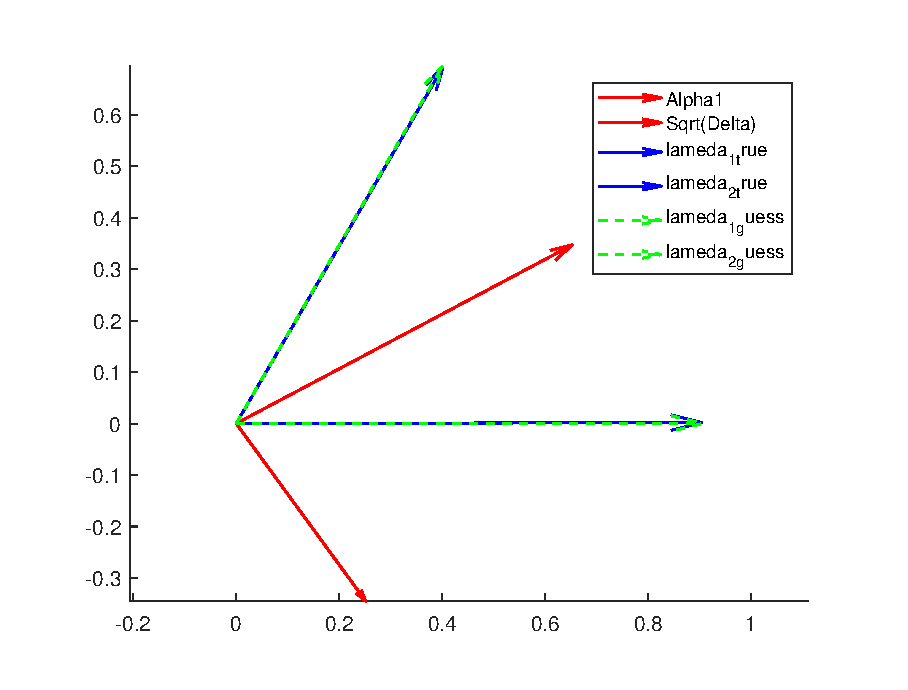
\includegraphics[scale=0.2]{1233.eps}
    \caption{figure title}
    \label{figure}
\end{figure}
    

\section{Multiple angle detection}

Let us get back to the general case and consider $(\hat \U_S^\H \J_1^\H \J_1 \hat \U_S )^{-1} \cdot \hat \U_S^\H \J_1^\H \J_2 \hat \U_S$. Note that the two matrices of interest are of small dimensions ($k \times k$) and can be shown to also establish asymptotically deterministic behavior.

In the case of a fixed number $k$ of signal sources with angle $\theta_1, \ldots, \theta_k$, we have the following generic model
\begin{equation}
	\X = \A \S + \Z 
\end{equation}
with $\X = [\x(1), \ldots, \x(T)] \in \CC^{N \times T}$, $\A = [\mathbf{a}(\theta_1), \ldots, \mathbf{a}(\theta_k)] \in \CC^{N \times k}$, $\S = [\s(1), \ldots, \s(T)] \in \CC^{k \times T}$, column vector $\s(t) = [s_1(t), \ldots, s_k(t)]^\T \in \CC^k$ and $\Z = [\z(1), \ldots, \z(T)] \in \CC^{N \times T}$ a standard (circular) Gaussian random matrix.
% "D:\Microsoft VS Code\Code.exe" "D:\Microsoft VS Code\resources\app\out\cli.js"  --ms-enable-electron-run-as-node -r -g "%f:%l"
As a consequence,
\begin{equation}
	\frac1T \X \X^\H = \frac1T \Z \Z^\H + \begin{bmatrix}\A & \frac{\Z \S^\H}{T}\end{bmatrix} \begin{bmatrix} \frac1T \S \S^\H & \I_k \\ \I_k & \mathbf{0}_k \end{bmatrix} \begin{bmatrix} \A^\H \\ \frac{(\Z \S^\H)^\H}{T}\end{bmatrix} \equiv \frac1T \Z \Z^\H + \V \bLambda \V^\H
\end{equation}
where we assume the the signals are uncorrelated and denote the diagonal $\mathbf{P} = \lim_{T\to \infty} \frac1T \S \S^\H$ the (limit of the normalized) signal strength and $\V = \begin{bmatrix}\A & \frac{\Z \S^\H}{T} \end{bmatrix} \in \CC^{N \times 2k}$.

As a consequence, 
\begin{align*}
	\left(\frac1T \X \X^\H - z \I_N \right)^{-1} &= \left(\frac1T \Z \Z^\H + \V \bLambda \V^\H - z \I_N \right)^{-1} \\ 
	&= \Q - \Q \V \bLambda (\I_{2k} + \V^\H \Q \V \bLambda)^{-1} \V^\H \Q
\end{align*}
where we denoted $\Q(z) = \Q = (\frac1T \Z \Z^\H - z \I_N)^{-1}$ and used Woodbury matrix identity. Now, since
\begin{equation}
	\V^\H \Q(z) \V = \begin{bmatrix}\A^\H \\ \frac{(\Z \S^\H)^\H}{T}\end{bmatrix} \Q(z) \begin{bmatrix} \A & \frac{\Z \S^\H}{T}\end{bmatrix} = \begin{bmatrix} \A^\H \Q(z) \A & \mathbf{0} \\ \mathbf{0} & \frac1T \S \frac1T \Z^\H \Q(z) \Z \S^\H \end{bmatrix} + o_{\| \cdot \|}(1)
\end{equation}
with
\begin{equation}
	\frac1T \S \frac1T \Z^\H \Q(z) \Z \S^\H = \frac1T \S \tilde \Q(z) \frac1T \Z^\H \Z \S^\H = \frac1T \S (\I_T + z \tilde \Q(z)) \S^\H = \mathbf{P} + \frac{z}T \S \tilde \Q(z) \S^\H
\end{equation}
for co-resolvent $\tilde \Q(z) = \left( \frac1T \Z^\H \Z - z \I_T \right)^{-1}$.

Since
\begin{equation}
	\Q(z) \leftrightarrow \bar \Q(z) = m(z) \I_N = \left(  \frac1{1 + c m(z)} - z \right)^{-1} \I_N, \quad \tilde \Q(z) = - \left(\frac1{z m(z)}+1\right) \I_T
\end{equation}
for $c = \lim N/T$ and $m(z)$ the unique solution of the Mar{\u c}enko-Pastur equation
\begin{equation}
	z c m^2(z) - (1 - c -z) m(z) + 1 = 0,
\end{equation}
Therefore
\begin{equation}
	(\I_{2k} + \V^\H \Q \V \bLambda)^{-1} = \begin{bmatrix} \I_k + m(z) \A^\H \A \mathbf{P} & m(z) \A^\H \A  \\ \left( 1 - z - \frac1{m(z)} \right) \mathbf{P} & \I_k  \end{bmatrix}^{-1} + o_{\| \cdot \|}(1)
\end{equation}
and 
\begin{equation}
	\V \bLambda (\I_2 + \V^\H \Q \V \bLambda)^{-1} \V^\H = \begin{bmatrix}\A & \frac{\Z \S^\H}{T}\end{bmatrix} \begin{bmatrix} (z + \frac1{m(z)}) ( \mathbf{P}^{-1} + (z m(z) + 1) \A^\H \A  )^{-1} & \H \\ \H & \H \end{bmatrix} \begin{bmatrix}\A^\H \\ \frac{(\Z \S^\H)^\H}{T}\end{bmatrix} + o_{\| \cdot \|} (1)
\end{equation}
so that it suffices to evaluate the following expectations:
\begin{enumerate}
 	\item $\EE[\Q(z) \A (\cdot) \A^\H \Q(z)] = (z m^2(z) + m(z)) \A (\mathbf{P}^{-1} + (z m(z) + 1) \A^\H \A  )^{-1} \A^\H  + o_{\| \cdot \|}(1)$;
 	\item $\frac1T \EE[\Q(z) \mathbf{a} \S^\H \Z^\T \Q(z)] = o_{\| \cdot \|}(1)$ and it Hermitian transpose.
 \end{enumerate}
This thus allows to conclude that
\begin{equation}
	\left(\frac1T \X \X^\H - z \I_N \right)^{-1} \leftrightarrow m(z) \I_N - (z m^2(z) + m(z)) \A (\mathbf{P}^{-1} + (z m(z) + 1) \A^\H \A  )^{-1} \A^\H.
\end{equation}
With the simplification of $\A^\H \A = \I_k$ as $N \to \infty$ in the LUA setting, we have
\begin{equation}
	\left(\frac1T \X \X^\H - z \I_N \right)^{-1} \leftrightarrow m(z) \I_N - (z m^2(z) + m(z)) \A (\mathbf{P}^{-1} + (z m(z) + 1) \I_k  )^{-1} \A^\H.
\end{equation}

In particular, for $k=1$, the above relation becomes
\begin{equation}
	\left(\frac1T \X \X^\H - z \I_N \right)^{-1} \leftrightarrow m(z) \I_N - \frac{\rho m(z) (z m(z) + 1) }{ 1 + \rho(z m(z) + 1) } \mathbf{a a}^\H.
\end{equation}
for $\mathbf{P} = \rho$ and where we recall that $\mathbf{a}^\H \mathbf{a} = \| \mathbf{a} \|^2 = 1$.


\subsection{Asymptotic location of isolated eigenvalues}

The asymptotic location of (the possible) isolated eigenvalues correspond to $z \in \RR$ such that
\begin{equation}
	\det( \P^{-1} + (z m(z) + 1) \A^\H \A ) = 0 \Leftrightarrow \det( (z m(z) + 1)^{-1} \I_k +  \mathbf{P} \A^\H \A ) = 0
\end{equation}
where we used the fact that $\det(\P^{-1}) \neq 0$ and $z m(z) + 1 \neq 0$, that is, 
\begin{equation}
	\frac1{z m(z) + 1} = -\lambda_i(\mathbf{P} \A^\H \A) \Leftrightarrow zm (z) = -1 - \frac1{\lambda_i(\mathbf{P} \A^\H \A)}
\end{equation}
where $\lambda_i(\mathbf{P} \A^\H \A) \geq 0$ denotes the eigenvalues of $\mathbf{P} \A^\H \A$.

First note that the function $x \mapsto xm(x) = \int \frac{x}{t-x} \mu(dt)$ is increasing and that $xm(x) \to -1$ as $x \to \infty$. Using the Mar\u{c}enko-Pastur equation
\begin{equation}\label{eq:MP-ST}
	zcm^2(z)-(1-c-z)m(z)+1=0 \Leftrightarrow zm(z) = -1 + \frac1{1-z-czm(z)}
\end{equation}
we particularly obtain $\lim_{x \downarrow (1+\sqrt c)^2} xm(x) = - 1 - \frac1{\sqrt c}$. So one must have $\ell_i = \lambda_i(\mathbf{P} \A^\H \A) \geq \sqrt c$. \textbf{This is the so-called separation condition}. Plugging $xm(z) = -1 - \frac1{\ell_i}$ back into \eqref{eq:MP-ST}, one deduces
\begin{equation}
	\hat \lambda_i \to \bar \lambda_i = 1 + \ell_i + c \frac{1+\ell_i}{\ell_i}, \quad \ell_i \equiv \lambda_i(\mathbf{P} \A^\H \A) \geq \sqrt c.
\end{equation}




\medskip

This can be (equivalently) derived by considering, for $z \in \RR$,
\begin{align*}
		0 = \det \left( \frac1T \X \X^\H - z \I_N  \right) = \ldots
\end{align*}


\subsection{ESPRIT performance analysis}


To analyze the performance of the ESPIRIT method, one needs to evaluate the following quantities
\begin{equation}
	T_1 = \A^\H \hat \uu_i \hat \uu_i^\H \A = (\A^\H \hat \uu_i) (\A^\H \hat \uu_i)^\H \in \CC^{k \times k}, \quad T_2 = \A^\H \hat \uu_i \hat \uu_i^\H \M \hat \uu_j \hat \uu_j^\H \A \in \CC^{k \times k}.
\end{equation}

Let us first consider the term $T_1$. For $(\hat \lambda_i, \hat \uu_i)$ an isolated eigenvalue-eigenvector pair of $\frac1n \X \X^\H$ (so in particular, one must have $\ell_i = \lambda_i(\mathbf{P} \A^\H \A) \geq \sqrt c$). Then, by Cauchy's integral formula
\begin{align}
	T_1 &= -\frac1{2\pi \imath} \oint_{\Gamma_{\bar \lambda_i}} \A^\H \left(\frac1T \X \X^\H - z \I_N \right)^{-1} \A \,dz = -\frac1{2\pi \imath}  \oint_{\Gamma_{\bar \lambda_i}} m(z) \A^\H \A \,dz \\ 
	 &+\frac1{2\pi \imath}  \oint_{\Gamma_{\bar \lambda_i}} m(z) (z m(z) + 1) \A^\H \A (\mathbf{P}^{-1} + (z m(z) + 1) \A^\H \A  )^{-1} \A^\H \A \,dz + o(1) \\ 
	 &= -\frac1{2\pi \imath}  \oint_{\Gamma_{\bar \lambda_i}} m(z) \left( \I_k + (z m(z) +1) \mathbf{P}^{\frac12} \A^\H \A \mathbf{P}^{\frac12} \right)^{-1}\A^\H \A \,dz + o(1) \\ 
	 &= {\rm Res}_{\bar \lambda_i} -m(z) \left( \I_k + (z m(z) +1) \mathbf{P}^{\frac12} \A^\H \A \mathbf{P}^{\frac12} \right)^{-1}\A^\H \A + o(1)
\end{align}
for $\Gamma_{\bar \lambda_i}$ a positively oriented contour circling around the asymptotic location of the $i$-th eigenvalue $\hat \lambda_i$. It thus suffices to consider the eigendecomposition of $\mathbf{P}^{\frac12} \A^\H \A \mathbf{P}^{\frac12} = \U \bLambda \U^\H$ and
% \begin{align*}
% 		T_1 &= {\rm Res}_{\bar \lambda_i} \U \diag \left\{ \frac{-m(z)}{ 1 + ( z m(z) + 1) \ell_j } \right\}_{j=1}^k \U^\H \A^\H \A + o_{\| \cdot \|}(1) \\ 
% 		&= \U \diag \left\{ \frac{-m(\bar \lambda_i)}{ \ell_j ( m(\bar \lambda_i) + \bar \lambda_i m'(\bar \lambda_i) )} \right\}_{j=1}^k \U^\H \A^\H \A + o_{\| \cdot \|}(1) \\ 
% 		& = - \frac{m(\bar \lambda_i)}{ m(\bar \lambda_i) + \bar \lambda_i m'(\bar \lambda_i) } \left( \mathbf{P}^{\frac12} \A^\H \A \mathbf{P}^{\frac12} \right)^{-1}\A^\H \A + o_{\| \cdot \|}(1).
% \end{align*}
\begin{align*}
		T_1 &= {\rm Res}_{\bar \lambda_i} \U \diag \left\{ \frac{-m(z)}{ 1 + ( z m(z) + 1) \ell_j } \right\}_{j=1}^k \U^\H \A^\H \A + o_{\| \cdot \|}(1) \\ 
		&= \frac{-m(\bar \lambda_i)}{ \ell_i ( m(\bar \lambda_i) + \bar \lambda_i m'(\bar \lambda_i) )} \uu_i \uu_i^\H \A^\H \A + o_{\| \cdot \|}(1).
\end{align*}
We in fact only care about the diagonal entries of $T_1$.

In the case of diagonal $\A^\H \A = \I_k$ (in the case of LUA), one obtains in particular,
\begin{equation}
	T_1 = - \frac{m(\bar \lambda_i)}{ \ell_i (m(\bar \lambda_i) + \bar \lambda_i m'(\bar \lambda_i)) } \uu_i \uu_i^\H + o_{\| \cdot \|}(1).
\end{equation}
In the special case uncorrelated sources with diagonal $\mathbf{P} = \diag\{ P_{\ell \ell} \}_{\ell=1}^k$, the $\uu_i$ are canonical vectors $\ee_i$ and
\begin{equation}
	[T_1]_{\ell \ell} = - \frac1{P_{\ell \ell}} \frac{m(\bar \lambda_i)}{ m(\bar \lambda_i) + \bar \lambda_i m'(\bar \lambda_i) }.
\end{equation}

% Also, the quantity $\tilde T_1 = \A^\T \hat \uu_i \uu_i^\H \A = $ can be similarly evaluated as

% And a consequence, interested in the ($k$-dimensional) complex random vector $\A^\H \hat \uu_i = A + \imath B$, we have the following equations
% \begin{equation}
% 	\A^\H \hat \uu_i \hat \uu^\H \A =  (A+ \imath B) (A - \imath B)^\T = A A^\T + B B^\T, \quad \A^\T \hat \uu_i \hat \uu^\H \A = \overline{\A^\H \hat \uu_i} \hat \uu^\H \A
% \end{equation}

\medskip

Let us move on and consider the (slightly) more involved term $T_2$. First note that, from the derivation of $T_1$, we have, for $\mathbf{a}, \mathbf{b}$ \emph{any} ($i'$-th and $j'$-th) column of $\A$ that
\begin{equation}
	\mathbf{a}^\H \hat \uu_i \hat \uu_i^\H \mathbf{b} = [T_1]_{i'j'} = - \frac{m(\bar \lambda_i)}{ \ell_i (m(\bar \lambda_i) + \bar \lambda_i m'(\bar \lambda_i)) } [\uu_i \uu_i^\H]_{i'j'} + o(1).
\end{equation}
Our objective is to, for any $\mathbf{a},\mathbf{b}$, estimate the \emph{complex} numbers $\mathbf{a}^\H \hat \uu_i$ and $\mathbf{b}^\H \hat \uu_i$.

For the convenience of further use, we can similarly derive
\begin{equation}
	\A^\T \hat \uu_i \hat \uu_i^\H \bar{\A} = \A^\T \bar{\hat \uu}_i {\bar \hat \uu}_i^\H \bar{\A}
\end{equation}


\section{MUSIC and its extension in random linear array setting}

In this section, we consider the more realistic Random Linear Array (RLA) setting of same $N$, which differs from the ULA setting \eqref{eq:def_ULA} in the fact that the steering vector $\mathbf{a}(\theta_\ell)$ of source $\ell$ and of arriving angle $\theta_\ell$ is now given by\footnote{The normalization by $\sqrt N$ here is for notational convenience so that $\mathbf{a}(\theta_\ell)$ is of unit norm, note that this is equivalent to a \emph{rescaling} of the source signal $s_\ell$.}
\begin{equation}
	[\mathbf{a}_{\bepsilon}(\theta_\ell)]_j = \frac1{\sqrt N} e^{\imath \frac{2\pi d_j}{\lambda_0} \sin(\theta_\ell)} = \frac1{\sqrt N} e^{\imath \frac{2\pi d (j-1)}{\lambda_0} \sin(\theta_\ell)} \cdot e^{\imath \frac{2\pi d \epsilon_j}{\lambda_0} \sin(\theta_\ell)} = \frac1{\sqrt N} e^{\imath (j-1) \omega \sin(\theta_\ell)} \cdot e^{\imath \omega \epsilon_j \sin(\theta_\ell)}
	%\frac1{\sqrt N} e^{\imath \omega (j-1) \sin(\theta_\ell)}, 
\end{equation}
for $\omega \equiv \frac{2 \pi d }{\lambda_0}$.
More precisely, the ``spacing'' $d_j$ between different receivers are no longer assumes to be strictly uniform, but only ``close to'' uniform such that
\begin{equation}
	d_j = (j-1) d + d \epsilon_j, \quad \epsilon_j \overset{i.i.d.}{\sim} \mathcal N(0, \sigma^2)
\end{equation}
with some small perturbation $\epsilon_j$ of zero mean and variance $\sigma^2$. As a consequence, we have
\begin{equation}
	\mathbf{a}_{\bepsilon}(\theta_\ell) = \mathbf{a}(\theta_\ell) \odot e^{\imath \omega \sin(\theta_\ell) \bepsilon }
\end{equation}
for the (standard) ULA steering vector $\mathbf{a}(\theta_\ell)$ defined in \eqref{eq:def_ULA}. Let us consider the following Taylor expansion of the nonlinear complex function $\exp(\imath \omega \sin \theta_\ell \cdot \epsilon )$ for $\epsilon \sim \mathcal N(0, \sigma^2) \ll 1$ (so in essence the assumption should be $\sigma^2  = o(1)$):
\begin{align}
	\exp(\imath \omega \sin \theta_\ell \cdot \epsilon ) &= 1 + \imath \omega \sin \theta_\ell \epsilon - \frac12 \omega^2 \sin^2 \theta_\ell \epsilon^2 - \frac{\imath}6 \omega^3 \sin^3 \theta_\ell \epsilon^3 + o(\epsilon^3) \\ 
	&= 1 - \frac12 \omega^2 \sin^2 \theta_\ell \epsilon^2 + \imath \cdot \omega \sin \theta_\ell \epsilon \cdot \left( 1 - \frac16 \omega^2 \sin^2 \theta_\ell \epsilon^2 \right) + o(\epsilon^3)
\end{align}
(Note interestingly that the approximation resulting from Taylor expansion entails that the expression is, in its first order, real.)
%where there is in total $k$ signal sources $\{s_{\ell}\}_{\ell=1}^k$, at angle $\{\theta_\ell\}_{\ell=1}^k$ for some $k \ll \min(N,T)$, as well as some independent Gaussian noise $\z(t) \overset{i.i.d.}{\sim} \mathcal{CN}(\zo, \I_N)$ for all $t$.

We consider again the following model for the signal received at time $t= 1,\ldots, T$
\begin{equation}
	\x(t) = \sum_{\ell = 1}^k \mathbf{a}_{\bepsilon}(\theta_\ell) s_\ell(t) + \z(t) = \sum_{\ell = 1}^k \mathbf{a}(\theta_\ell) \odot e^{\imath \omega \sin(\theta_\ell) \bepsilon } \cdot s_\ell(t) + \z(t) \in \CC^N
\end{equation}
which can be rewritten in matrix model by cascading the total $T$ observations as  
\begin{equation}
	\X = \A_{\bepsilon} \S + \Z = \left( \A \odot [e^{\imath \omega \sin(\theta_1) \bepsilon }, \ldots, e^{\imath \omega \sin(\theta_k) \bepsilon }] \right) \S + \Z
\end{equation}
with $\X = [\x(1), \ldots, \x(T)] \in \CC^{N \times T}$, $\A_{\bepsilon} = [\mathbf{a}_{\bepsilon}(\theta_1), \ldots, \mathbf{a}_{\bepsilon}(\theta_k)] \in \CC^{N \times k}$, $\S = [\s(1), \ldots, \s(T)] \in \CC^{k \times T}$, column vector $\s(t) = [s_1(t), \ldots, s_k(t)]^\T \in \CC^k$ and $\Z = [\z(1), \ldots, \z(T)] \in \CC^{N \times T}$ a standard (circular) Gaussian random matrix.

\subsection{Simplified model with single DoA}

In the case of $k=1$ with angle $\theta$, we have the following simplified model
\begin{equation}
	\X = \mathbf{a}_{\bepsilon}(\theta) [s(1), \ldots, s(T)] + \Z \equiv \mathbf{a}_{\bepsilon}(\theta) \s^\H + \Z
\end{equation}
so that 
\begin{equation}
	\frac1T \X \X^\H = \frac1T \Z \Z^\H + \begin{bmatrix}\mathbf{a}_{\bepsilon} & \frac{\Z \s}{T}\end{bmatrix} \begin{bmatrix} \rho & 1 \\ 1 & 0 \end{bmatrix} \begin{bmatrix}\mathbf{a}_{\bepsilon}^\H \\ \frac{(\Z \s)^\H}{T}\end{bmatrix} \equiv \frac1T \Z \Z^\H + \V \bLambda \V^\H
\end{equation}
where we denote $\rho = \frac1T \| \s \|^2 $ the (limit of the normalized) signal strength and $\V = \begin{bmatrix}\mathbf{a}_{\bepsilon} & \frac{\Z \s}{T}\end{bmatrix} \in \CC^{N \times 2}$. Taking the expectation with respect to $\Z$, one obtains
\begin{equation}
	\frac1T \EE_\X[\X \X^\H] = \I_N + \rho \cdot \mathbf{a}_{\bepsilon} \mathbf{a}_{\bepsilon}^\H
\end{equation}
further taking the expectation with respect to $\bepsilon$, the (i,j) entry of which is given by
\begin{align}
	\frac1T \EE[\X \X^\H]_{ij} &= \delta_{ij} + \frac{\rho}N e^{\imath (i-1) \omega \sin(\theta)} \cdot e^{-\imath (j-1) \omega \sin(\theta)} \cdot \EE [e^{\imath \omega \epsilon_i \sin(\theta)} \cdot e^{-\imath \omega \epsilon_j \sin(\theta)}] \\ 
	& =\delta_{ij} + \frac{\rho}N e^{\imath (i-1) \omega \sin(\theta)} \cdot e^{-\imath (j-1) \omega \sin(\theta)} \cdot e^{-\frac12 \omega^2 \sigma^2 \sin^2 \theta} \cdot e^{-\frac12 \omega^2 \sigma^2 \sin^2 \theta} \\ 
	& = \delta_{ij} + \frac{\rho}N e^{\imath (i-1) \omega \sin(\theta)} \cdot e^{-\imath (j-1) \omega \sin(\theta)} \cdot e^{-\omega^2 \sigma^2 \sin^2 \theta}
\end{align}
for $i \neq j$, so that 
\begin{equation}
	\frac1T \EE[\X \X^\H] = (1 +  \frac{\rho}N - \frac{\rho}N e^{- \omega^2 \sigma^2 \sin^2 \theta} ) \I_N + \frac{\rho}N \mathbf{a} \mathbf{a}^\H \cdot e^{-\omega^2 \sigma^2 \sin^2 \theta}
\end{equation}
{\BLUE simulation seems OK.}

It can be further checked that 
\begin{equation}
	\lambda_1(\EE[\X \X^\H] /T) = 1 + \frac{\rho}{N}
\end{equation}
that is, the MUSIC method is \emph{robust} in the random linear array setting, in the sense that its performance is independent of the noise level. {\BLUE The same conclusion can be reached by a RMT analysis, from which the MUSIC performance can be shown to only depend on the eigenvalue of $\A \mathbf{P} \A^\H$, and not the specific form of the steering vector $\mathbf{a}$. }


\section{ESPIRIT approach in random linear array setting}


\bibliography{liao}
\bibliographystyle{plain}
\end{document}